% ***************************************************************************************************
%
%	Szablon pracy magisterskiej dla Politechniki Wrocławskiej w wersji dwustronnej.
%	Autor:	Tomasz Strzałka
%
% ***************************************************************************************************

% Styl dwustronny z domyślną wielkością czcionki 10pt oraz oddzieloną stroną tytułową (titlepage).
% Domyślnie rodziały rozpoczynają się na stronie prawej (openright).
\documentclass{book}

% ***************************************************************************************************
% Ustawienia języka
% ***************************************************************************************************

% Podstawowe ustawienia języka, według którego formatowany będzie dokument
\usepackage[polish]{babel}

% Pakiet babel dla polskiego języka powoduje konflikt z pakietem amssymb.
% Polecenie '\lll' definiują oba pakiety - porządana jest druga definicja.
\let\lll\undefined

% W przypadku wielojęzykowości ustawia główny język dokumentu
\selectlanguage{polish}

% Kodowanie dokumentu
\usepackage[utf8]{inputenc}

% Dowolny rozmiar czcionek, kodowanie znaków
\usepackage{lmodern}

% Polskie wcięcia akapitów
\usepackage{indentfirst}

% Polskie łamanie wyrazów
\usepackage[plmath]{polski}

% Przecinek w wyrażeniach matematycznych zamiast kropki
\usepackage{icomma}

% Polskie formatowanie typograficzne
\frenchspacing

% Zapewnia liczne usprawnienia wyświetlania i organizacji matematycznych formuł. 
\usepackage{amsmath}

% Wprowadza rozszerzony zestaw symboli m.in. \leadsto
\usepackage{amssymb}

% Dodatkowa, ,,kręcona'' czcionka matematyczna
\usepackage{mathrsfs}

% Dodatkowe wsparcie dla środowiska mathbb, które nie wspiera domyślnie cyfr (\mathbb{})
\usepackage{bbold}

% Fixes/improves amsmath
\usepackage{mathtools}

\usepackage{float}
\usepackage{wrapfig}


% ***************************************************************************************************
% Kolory  
% ***************************************************************************************************

% Umożliwia kolorowanie poszczególnych komórek tabeli
\usepackage[table]{xcolor}% http://ctan.org/pkg/

% Umożliwia łatwą zmianę koloru linii w tabeli
\usepackage{tabu}

% Umożliwia rozszerzoną kontrolę nad kolorami.
\usepackage{xcolor}

% Definicje kolorów
\definecolor{lgray}{HTML}{9F9F9F}
\definecolor{dgray}{HTML}{5F5F5F}
% lgray				-	nazwa nowo zdefiniowanego koloru
% HTML				-	model kolorów
% CCCCCC			-	wartość koloru zgodna z modelem

% ***************************************************************************************************
% Algorytmy 
% ***************************************************************************************************

% Udostępnia środowisko do konstruowania pseudokodów
%\usepackage[ruled,vlined,linesnumbered,longend,algochapter]{algorithm2e}
% ruled	- poziome kreski na początku i końcu algorytmu, podpis na górze oddzielony również kreską poziomą
% vlined - pionowe kreski łączące początek polecenia z jego końcem
% linesnumbered	- numerowanie kolejnych wierszy algorytmu
% longend - długie końcówki np. ifend, forend itd.
% algochapter - numeracja z rozdziałami

% Zamiana nazwy środowiska z domyślnej "Algorithm X" na "Pseudokod X"
%\newenvironment{pseudokod}[1][htb]{
%	\renewcommand{\algorithmcfname}{Pseudokod}
%	\begin{algorithm}[#1]%
%	}{
%\end{algorithm}
%}

% Zmiana rozmiaru komentarzy
%\newcommand\algcomment[1]{
%	\footnotesize{#1}
%}

% Ustawienie zadanego stylu dla komentarzy
%\SetCommentSty{algcomment}

% Wyśrodkowana tylda
\usepackage{textcomp}%
\newcommand{\textapprox}{\raisebox{0.5ex}{\texttildelow}}

% Listowanie kodów źródłowych
\usepackage{listings} 
\renewcommand{\lstlistingname}{Kod źródłowy} % Polska nazwa listingu

% Definicje pecjalnych znaków, które nie są obsługiwane w środowisku listing
\lstset{literate=
	{ż}{{\.{z}}}1	{ź}{{\'{z}}}1
	{ć}{{\'{c}}}1	{ń}{{\'{n}}}1
	{ą}{{\c a}}1	{ś}{{\'{s}}}1
	{ł}{{\l}}1		{ę}{{\c{e}}}1
	{ó}{{\'{o}}}1	{á}{{\'a}}1
	{é}{{\'e}}1		{í}{{\'i}}1
	{ó}{{\'o}}1		{ú}{{\'u}}1
	{ù}{{\`u}}1		{Á}{{\'A}}1
	{É}{{\'E}}1		{Í}{{\'I}}1
	{Ó}{{\'O}}1		{Ú}{{\'U}}1
	{à}{{\`a}}1		{è}{{\'e}}1
	{ì}{{\`i}}1		{ò}{{\`o}}1
	{ò}{{\`o}}1		{À}{{\`A}}1
	{È}{{\'E}}1		{Ì}{{\`I}}1
	{Ò}{{\`O}}1		{Ò}{{\`O}}1
	{ä}{{\"a}}1		{ë}{{\"e}}1
	{ï}{{\"i}}1		{ö}{{\"o}}1
	{ü}{{\"u}}1		{Ä}{{\"A}}1
	{Ë}{{\"E}}1		{Ï}{{\"I}}1
	{Ö}{{\"O}}1		{Ü}{{\"U}}1
	{â}{{\^a}}1		{ê}{{\^e}}1
	{î}{{\^i}}1		{ô}{{\^o}}1
	{û}{{\^u}}1		{Â}{{\^A}}1
	{Ê}{{\^E}}1		{Î}{{\^I}}1
	{Ô}{{\^O}}1		{Û}{{\^U}}1
	{œ}{{\oe}}1		{Œ}{{\OE}}1
	{æ}{{\ae}}1		{Æ}{{\AE}}1
	{ß}{{\ss}}1		{ç}{{\c c}}1
	{Ç}{{\c C}}1	{ø}{{\o}}1
	{å}{{\r a}}1	{Å}{{\r A}}1
	{€}{{\EUR}}1	{£}{{\pounds}}1
}

% ***************************************************************************************************
% Marginesy 
% ***************************************************************************************************

% Ustawienia rozmiarów stron i ich marginesów
\usepackage[headheight=18pt, top=25mm, bottom=25mm, left=25mm, right=25mm]{geometry}
% headheight		-	wysokość tytułów
% top				-	margines górny
% bottom			-	margines dolny
% left				-	margines lewy
% right				-	margines prawy

% Usunięcie górnego marginesu dla środowisk
\makeatletter
\setlength\@fptop{0\p@}	
\makeatother

% ***************************************************************************************************
% Styl 
% ***************************************************************************************************

% Definiuje środowisko 'titlingpage', które zapewnia pełną kontrolę nad układem strony tytułowej.
\usepackage{titling}


% Umożliwia modyfikowanie stylu spisu treści
\usepackage{tocloft}	

\tocloftpagestyle{tableOfContentStyle}

% Definiowanie własnych stylów nagłówków i/lub stopek
\usepackage{fancyhdr}

% Domyślny styl dla pracy 
\fancypagestyle{custom}{
	\fancyhf{}									% wyczyść stopki i nagłówki
	\fancyhead[RO]{								% Prawy, nieparzysty nagłówek
		\hrulefill \hspace{16pt} \large Rozdział \thechapter
		\put(-472.1, 12.1){%
			\makebox(0,0)[l]{%
				
\includegraphics[width=0.05\textwidth]{pwr-logo}
			}
		}
		\put(-443,5.5){%
			\makebox(0,0)[l]{%
				\small Politechnika Wrocławska
			}
		}
	}
	\fancyhead[LE]{								% Lewy, parzysty nagłówek
		\large Rozdział \thechapter \hspace{16pt} \hrulefill 
		\put(-22, 12.1){%
			\makebox(0,0)[l]{%
				
\includegraphics[width=0.05\textwidth]{wppt-logo}
			}
		}
		\put(-210,5.5){%
			\makebox(0,0)[l]{%
				\small Wydział Podstawowych Problemów Techniki
			}
		}
	}
	\fancyfoot[LE,RO]{							% Stopki
		\thepage
	}
	\renewcommand{\headrulewidth}{0pt}			% Grubość linii w nagłówku
	\renewcommand{\footrulewidth}{0.2pt}		% Grubość linii w stopce
}


% Domyślny styl dla bibliografii
\fancypagestyle{bibliographyStyle}{
	\fancyhf{}									% wyczyść stopki i nagłówki
	\fancyhead[RO]{								% Prawy, nieparzysty nagłówek
		\hrulefill \hspace{16pt} \large Dodatek \thechapter
		\put(-472.1, 12.1){%
			\makebox(0,0)[l]{%
				
\includegraphics[width=0.05\textwidth]{pwr-logo}
			}
		}
		\put(-443,5.5){%
			\makebox(0,0)[l]{%
				\small Politechnika Wrocławska
			}
		}
	}
	\fancyhead[LE]{								% Lewy, parzysty nagłówek
		\large Bibliografia \hspace{16pt} \hrulefill 
		\put(-22, 12.1){%
			\makebox(0,0)[l]{%
				
\includegraphics[width=0.05\textwidth]{wppt-logo}
			}
		}
		\put(-210,5.5){%
			\makebox(0,0)[l]{%
				\small Wydział Podstawowych Problemów Techniki
			}
		}
	}
	\fancyfoot[LE,RO]{							% Stopki
		\thepage
	}
	\renewcommand{\headrulewidth}{0pt}			% Grubość linii w nagłówku
	\renewcommand{\footrulewidth}{0.2pt}		% Grubość linii w stopce
}

% Domyślny styl dla dodatków
\fancypagestyle{appendixStyle}{
	\fancyhf{}									% wyczyść stopki i nagłówki
	\fancyhead[RO]{								% Prawy, nieparzysty nagłówek
		\hrulefill \hspace{16pt} \large Dodatek \thechapter
		\put(-472.1, 12.1){%
			\makebox(0,0)[l]{%
				
\includegraphics[width=0.05\textwidth]{pwr-logo}
			}
		}
		\put(-443,5.5){%
			\makebox(0,0)[l]{%
				\small Politechnika Wrocławska
			}
		}
	}
	\fancyhead[LE]{								% Lewy, parzysty nagłówek
		\large Dodatek \thechapter \hspace{16pt} \hrulefill 
		\put(-22, 12.1){%
			\makebox(0,0)[l]{%
				
\includegraphics[width=0.05\textwidth]{wppt-logo}
			}
		}
		\put(-210,5.5){%
			\makebox(0,0)[l]{%
				\small Wydział Podstawowych Problemów Techniki
			}
		}
	}
	\fancyfoot[LE,RO]{							% Stopki
		\thepage
	}
	\renewcommand{\headrulewidth}{0pt}			% Grubość linii w nagłówku
	\renewcommand{\footrulewidth}{0.2pt}		% Grubość linii w stopce
}

% Osobny styl dla stron zaczynających rozdział/spis treści itd. (domyślnie formatowane jako "plain")
\fancypagestyle{chapterBeginStyle}{
	\fancyhf{}%
	\fancyfoot[LE,RO]{
		\thepage
	}
	\renewcommand{\headrulewidth}{0pt}
	\renewcommand{\footrulewidth}{0.2pt}
}

% Styl dla pozostałych stron spisu treści
\fancypagestyle{tableOfContentStyle}{
	\fancyhf{}%
	\fancyfoot[LE,RO]{
		\thepage
	}
	\renewcommand{\headrulewidth}{0pt}
	\renewcommand{\footrulewidth}{0.2pt}
}

% Formatowanie tytułów rozdziałów i/lub sekcji
\usepackage{titlesec}

% Formatowanie tytułów rozdziałów
\titleformat{\chapter}[hang]					% kształt
{
	\vspace{-10ex}
	\Huge
	\bfseries
}												% formatowanie tekstu modyfikowanego elementu
{}												% etykieta występująca przed tekstem modyfikowanego elementu, niewidoczna w spisie treści
{
	10pt
}												% odstęp formatowanego tytułu od lewego marginesu/etykiety
{
	\Huge
	\bfseries
}												% formatowanie elementów przed modyfikowanym tytułem
[
\vspace{2ex}
%\rule{\textwidth}{0.4pt}
%\vspace{-4ex}
]												% dodatkowe formatowanie stosowane poniżej modyfikowanego tytułu


% Formatowanie tytułów sekcji
\titleformat{\section}[hang]					% kształt
{
	\vspace{2ex}
%	\titlerule\vspace{1ex}
	\Large\bfseries
}												% formatowanie tekstu modyfikowanego elementu
{
	\thesection									% etykieta występująca przed tekstem modyfikowanego elementu, niewidoczna w spisie treści
}
{
	0pt
}												% odstęp formatowanego tytułu od lewego marginesu/etykiety
{
	\Large
	\bfseries
}												% formatowanie elementów przed modyfikowanym tytułem

% ***************************************************************************************************
% Linki
% ***************************************************************************************************

% Umożliwia wstawianie hiperłączy do dokumentu
\usepackage{hyperref}							% Aktywuje linki

\hypersetup{
	colorlinks	=	true,					% Koloruje tekst zamiast tworzyć ramki.
	linkcolor		=	blue,					% Kolory: referencji,
        citecolor		=	blue,					% cytowań,
	urlcolor		=	blue					% hiperlinków.
}

% Do stworzenia hiperłączy zostanie użyta ta sama (same) czcionka co dla reszty dokumentu
\urlstyle{same}




% ***************************************************************************************************
% Linki
% ***************************************************************************************************

% Umożliwia zdefiniowanie własnego stylu wyliczeniowego
\usepackage{enumitem}

% Nowa lista numerowana z trzema poziomami
\newlist{myitemize}{itemize}{3}

% Definicja wyglądu znacznika pierwszego poziomu
\setlist[myitemize,1]{
	label		=	\textbullet,
	leftmargin	=	4mm}

% Definicja wyglądu znacznika drugiego poziomu
\setlist[myitemize,2]{
	label		=	$\diamond$,
	leftmargin	=	8mm}

% Definicja wyglądu znacznika trzeciego poziomu
\setlist[myitemize,3]{
	label		=	$\diamond$,
	leftmargin	=	12mm
}

% ***************************************************************************************************
% Inne pakiety
% ***************************************************************************************************

% Dołączanie rysunków
\usepackage{graphicx}

\graphicspath{ {}{images/} }

% Figury i przypisy
\usepackage{caption}
\usepackage{subcaption}

% Umożliwia tworzenie przypisów wewnątrz środowisk
\usepackage{footnote}

% Umożliwia tworzenie struktur katalogów
\usepackage{dirtree}

% Rozciąganie komórek tabeli na wiele wierszy
\usepackage{multirow}

% Precyzyjne obliczenia szerokości/wysokości dowolnego fragmentu wygenerowanego przez LaTeX
\usepackage{calc}

\usepackage{algorithm}
\usepackage{algpseudocode}

% ***************************************************************************************************
% Matematyczne skróty
% ***************************************************************************************************

% Skrócony symbol liczb rzeczywistych
\newcommand{\RR}{\mathbb{R}}

% Skrócony symbol liczb naturalnych
\newcommand{\NN}{\mathbb{N}}

% Skrócony symbol liczb wymiernych
\newcommand{\QQ}{\mathbb{Q}}

% Skrócony symbol liczb całkowitych
\newcommand{\ZZ}{\mathbb{Z}}

% Skrócony symbol logicznej implikacji
\newcommand{\IMP}{\rightarrow}

% Skrócony symbol  logicznej równoważności
\newcommand{\IFF}{\leftrightarrow}

% ***************************************************************************************************
% Środowiska
% ***************************************************************************************************

% Środowisko do twierdzeń
\newtheorem{theorem}{Twierdzenie}[chapter]

% Środowisko do lematów
\newtheorem{lemma}{Lemat}[chapter]

% Środowisko do przykładów
\newtheorem{example}{Przykład}[chapter]

% Środowisko do wniosków
\newtheorem{corollary}{Wniosek}[chapter]

% Środowisko do definicji
\newtheorem{definition}{Definicja}[chapter]

% Środowisko do dowodów
\newenvironment{proof}{
	\par\noindent \textbf{Dowód.}
}{
\begin{flushright}
	\vspace*{-6mm}\mbox{$\blacklozenge$}
\end{flushright}
}

% Środowisko do uwag
\newenvironment{remark}{
	\bigskip \par\noindent \small \textbf{Uwaga.}
}{
\begin{small}
	\vspace*{4mm}
\end{small}
}

% ***************************************************************************************************
% Słownik
% ***************************************************************************************************

% Prawidłowe dzielenie wyrazów
\hyphenation{wszy-stkich ko-lu-mnę każ-da od-leg-łość
	dzie-dzi-ny dzie-dzi-na rów-nych rów-ny
	pole-ga zmie-nna pa-ra-met-rów wzo-rem po-cho-dzi
	o-trzy-ma wte-dy wa-run-ko-wych lo-gicz-nie
	skreś-la-na skreś-la-ną cał-ko-wi-tych wzo-rów po-rzą-dek po-rząd-kiem
	przy-kład pod-zbio-rów po-mię-dzy re-pre-zen-to-wa-ne
	rów-no-waż-ne bi-blio-te-kach wy-pro-wa-dza ma-te-ria-łów
	prze-ka-za-nym skoń-czo-nym moż-esz na-tu-ral-na cią-gu tab-li-cy
	prze-ka-za-nej od-po-wied-nio}

% ***************************************************************************************************
% Dokument
% ***************************************************************************************************

\frontmatter

\newcommand{\JL}[1]{\marginpar{\small {\bf JL}: #1}}


\begin{document}

	\begin{titlingpage}
		\vspace*{\fill}
		\begin{center}
			\begin{picture}(300,510)
				\put(11,520){\makebox(0,0)[l]{\large \textsc{Wydział Podstawowych Problemów Techniki}}}
				\put(11,500){\makebox(0,0)[l]{\large \textsc{Politechnika Wrocławska}}}
% Tytuł pracy
				\put(80,320){\Huge \textsc{Analiza strumieni}}
				\put(80,280){\Huge \textsc{danych online}}
				\put(80,240){\Huge \textsc{}}
% Autor pracy
				\put(90,200){\makebox(0,0)[l]{\large \textsc{Adam Wilczak}}}
				\put(90,180){\makebox(0,0)[l]{\large \textsc{Nr indeksu: 204409}}}

				\put(200,100){\makebox(0,0)[l]{\large Praca magisterska napisana}}
				\put(200,80){\makebox(0,0)[l]{\large pod kierunkiem}}
% dane promotora
				\put(200,60){\makebox(0,0)[l]{\large dra Jakuba Lemiesza}}
				
				\put(115,-70){
\includegraphics[width=0.15\textwidth]{pwr}}
				\put(106,-80){\makebox(0,0)[bl]{\large \textsc{Wrocław 2017}}}
			\end{picture}
		\end{center}	
		\vspace*{\fill}
	\end{titlingpage}
	
        \cleardoublepage
		
	\pagenumbering{Roman}
	\pagestyle{tableOfContentStyle}
	\tableofcontents
	\cleardoublepage
		
	% ***************************************************************************************************
	% Wstęp
	% ***************************************************************************************************
	
	\pagestyle{custom}
	\mainmatter
	
	% ***************************************************************************************************
	% Rodziały
	% ***************************************************************************************************

	\chapter{Wstęp}
\thispagestyle{chapterBeginStyle}

W tej pracy podejmiemy temat przybliżonego zliczania unikalnych elementów w strumieniu danych w oparciu o efektywne szkice danych, a także możliwości wykorzystania tych szkiców do szacowania wyników operacji teoriomnogościowych na odpowiadających im danych.

Problem przybliżonego zliczania unikalnych elementów coraz częściej pojawia się w systemach przetwarzania danych i środowiskach OLAP (Online Analytical Data Processing).
W systemach tego typu bardzo często mamy do czynienia z masywnymi strumieniami danych, których dokładna  analiza wymaga dużych zasobów pamięciowych i obliczeniowych. W szczególności próba dokładnego zliczania unikalnych elementów w strumieniu jest związana z dużymi wymaganiami pamięciowymi,  gdyż wymaga przechowywania wszystkich napotkanych dotychczas różnych elementów.
Takie podejście wydaje się bardzo niewydajne,
zwłaszcza biorąc pod uwagę liczbę urządzeń oraz aplikacji generujących dziś dane 
oraz to,  w jak dużych ilościach i z jaką częstotliwością te dane napływają
(np. logi napływające w tysiącach wpisów na sekundę).
Często przechowywanie takich danych wymagałoby
setek terabajtów pamięci, a przestrzeń ta będzie szybko rosła z każdym kolejnym napływającym wpisem.

W odpowiedzi na powyższy problem zaproponowano wykorzystanie algorytmów probabilistycznych, które pozawalają oszacować liczbę unikalne elementy z pewnym kontrolowanym błędem, ale mają istotnie mniejsze wymagania pamięciowe. Algorytmy te operują na tak zwanych szkicach danych będących ich skrótową reprezentacją (np. w postaci haszy wybranych elementów). Jednym z pierwowzorów tego typu algorytmów był, oparty na idei liczników probabilistycznych, algorytm \textit{Probabilistic Counting} \cite{linear}. 
Jego idea została rozwinięta w algorytmie \textit{LogLog} \cite{loglog},
a ostatecznie znalazła zastosowanie w dobrze dziś znanym
algorytmie \textit{HyperLogLog} \cite{hll}.
Algorytm \textit{HyperLogLog} jest obecnie wykorzystywany i rozwijany m.in. przez firmy takie 
jak Google \cite{hllpp} czy Oracle \cite{oracle}.  

Inna, popularna rodzina algorytmów przybliżonego zliczania jest oparta na pomyśle związanym ze statystykami pozycyjnymi. Do tej rodziny należy m.in. znany pod kilkoma różnymi nazwami algorytm \textit{MinCount}, który szczegółowo omówimy w tej pracy. Oprócz tego istnieje jeszcze wiele innych algorytmów zliczania takich jak np. \textit{Multiresolution Bitmap, S-Bitmap czy MaxCount}
\cite{streamed}.

Niniejsza praca ma na celu omówieniem najbardziej popularnych algorytmów przybliżonego zliczania i rozważenie możliwości wykorzystania szkiców danych
na jakich się opierają do do przeprowadzania operacji teoriomnogościowych na zbiorach danych, z którymi są związane.  Możliwość wykonywanie operacji teoriomnogościowych na szkicach danych jest ostatnio przedmiotem wielu badań \cite{ting} \cite{oertl} \cite{adroll}.
Operacje teoriomnogościowych na szkicach ma wiele zastosowań praktycznych związanych z agregacją danych i  wykonywaniem  zapytań na wielu szkicach. Jako przykład rozważmy problem zliczania unikatowych użytkowników odwiedzających stronę internetową. Załóżmy, że średnio stronę odwiedza około 100 osób na sekundę i dokładne zliczanie unikalnych adresów IP jest zbyt kosztowne pamięciowo. Możemy użyć jednej z metod aproksymacyjnych do stworzenia szkiców odpowiadających unikalnym użytkownikom odwiedzających stronę  w ciągu każdej godziny. W przyszłości moglibyśmy być jednak zainteresowani innymi informacjami, np. ilu było
unikalnych użytkowników jednego dnia, jednego mieniąca
lub ilu jest użytkowników, którzy odwiedzają stronę rano i wieczorem.   
Wówczas możliwość wykonywania operacji sumowania, przekroju czy różnicy na szkicach umożliwiałaby wykorzystanie istniejących szkiców o małej granulacji czasowej i nie byłoby potrzeby tworzenia wielu szkiców o różnej granulacji czasowej. 

Zauważmy ponadto, że możliwość wykonywania operacji 
teoriomnogościowych na szkicach umożliwiałaby również
łatwe zliczanie unikalnych elementów w środowisku rozproszonym. Przykładowo, moglibyśmy podzielić masywny strumień danych na wiele podstrumieni przetwarzanych niezależnie na różnych węzłach klastra (osobne szkice)
a następnie zagregować informacje wykorzystując operacje sumy.

\subsubsection{Struktura pracy}
Praca jest podzielona na pięć rozdziałów. W rozdziale pierwszym omówimy popularne algorytmy przybliżonego zliczania: \textit{MinCount} oraz \textit{HyperLogLog}, a także związane z nimi szkice danych. 
W rozdziale drugim omówimy podstawowe techniki 
umożliwiające wykonywanie  teoriomnogościowych na szkicach danych. W rozdziale trzecim omówimy metodę \textit{estymatora ważonego} przedstawioną w \cite{ting} i umożliwiającą wykonywanie operacji sumy i przekroju na szkicach związanych z algorytmem \textit{MinCount}. Pokażemy także, jak można tę metodę uogólnić dla szkiców związanych z algorytmem \textit{HyperLogLog} oraz jak można ją zastosować do oszacowania rozmiaru różnicy szkiców. W rozdziale czwartym przedstawimy i omówimy wyniki eksperymentów, dokonując porównania przedstawionych wcześniej metod.
	\cleardoublepage

	\chapter{Algorytmy przybliżonego zliczania}
\thispagestyle{chapterBeginStyle}
\label{rozdzial1}

W tym rozdziale  opiszemy problem zliczania oraz trzy  algorytmy przybliżonego zliczania, na których będzie się opierała dalsza cześć pracy:  \texttt{MinCount},  \texttt{Streaming MinCount} oraz \texttt{HyperLogLog}. Omówimy ich działanie, związane z nimi szkice danych, a także obciążenie i koncentrację opartych na tych szkicach estymatorów. Przedstawimy również pełny kod algorytmów. 
%%JL Następnie omówimy także naiwne metody estymacji 
%%operacji teoriomnogościowych dla tych algorytmów.


\section{Problem zliczania}
Najpierw zdefiniujmy czym jest problem zliczania, którego dotyczy nasza praca.
Zacznijmy od zdefiniowania pojęcia \textit{multizbioru}. Multizbiór $\mathfrak{M}$ definiujmy jako parę $(S, m)$, gdzie $S$ jest zbiorem nazywanym \textit{zbiorem fundamentalnym} , natomiast $m$ jest funkcją postaci $m : S \rightarrow \mathbb{N}_{\geq 1}$. Wartość $m(s)$ nazywamy mnogością elementu $s \in S$. Problem zliczania możemy zatem sformułować w taki sposób: mając multizbiór $\mathfrak{M}$, znaleźć moc $n$ zbioru fundamentalnego $S$.

W ogólnym przypadku, nie posiadając żadnych informacji na temat danych, aby znaleźć dokładne rozwiązanie tego problemu potrzebujemy liniowej pamięci $O(n)$. Zatem, próba zmniejszenia zapotrzebowania pamięci algorytmu poniżej tego poziomu musi mieć wpływ na jego dokładność i skutkuje zmniejszeniem dokładności ostatecznego wyniku. Na szczęście jeśli jesteśmy w stanie kontrolować ten błąd i jest on stosunkowo niewielki - wówczas taki algorytm jest wystarczający w większości praktycznych zastosowań i daje nam satysfakcjonunjący wynik.


\section{Algorytm MinCount}

Pierwszym algorytmem przybliżonego zliczania, którym się zajmiemy jest \texttt{MinCount} znany również pod innymi nazwami, np.  \texttt{K-th Minimum Value} (KMV) \cite{kmv}. Algorytm ten opiera się na statystykach pozycyjnych.

\subsubsection{Statystyki pozycyjne}

Rozważmy  zmienne losowe $X_1, X_2, \dots, X_n$. Statystykami pozycyjnymi będziemy nazywać zmienne losowe  $X_{(1)}, X_{(2)}, \dots, X_{(n)}$ powstałe przez posortowanie realizacji zmiennych $X_1, X_2, \dots, X_n$ rosnąco.  Zmienną $X_{(k)}$ nazywamy k-tą statystyką pozycyjną. W szczególności $X_{(1)} = \min\{X_1, X_2, \dots, X_n \}$. W dalszej części pracy będziemy zakładać, że
zmienne $X_1, X_2, \dots X_n$ są niezależne i każda  ma rozkład jednostajny na odcinku (0,1).

Przyjmijmy, że istnieje funkcja haszująca 
\begin{equation}
    h \colon \mathfrak{M} \rightarrow (0, 1)
\end{equation}
taka, że jeśli $\mathfrak{M}$ posiada $n$ unikalnych elementów $a_1, a_2, \dots a_n$ to przyjmując, że
 $U_i = h(a_i)$ otrzymamy ciąg niezależnych zmiennych losowych o rozkładzie jednostajnym $U_1, U_2, \dots U_n \sim U(0,1)$. Zauważmy również, że jeśli element $a_i$ pojawia się w  $\mathfrak{M}$ wielokrotnie, to zawsze będzie zhaszowany do tej samej wartości.
 
Rozważmy statystyki pozycyjne  $U_{(1)}, U_{(2)}, \dots, U_{(n)}$ powstałe przez posortowanie realizacji  $U_1, U_2, \dots U_n$. O zmiennej losowej $U_{(k)}$ wiemy, że pochodzi z rozkładu $Beta(\alpha, \beta)$, gdzie $\alpha = k, \beta = n + 1 - k$ i jest zdefiniowana przez następującą funkcję rozkładu prawdopodobieństwa \cite{mincount}:
\begin{equation}
    f(x; \alpha, \beta) = \frac{x^{\alpha-1}{(1-x)}^{\beta-1}}{B(\alpha, \beta)},
\end{equation} 
gdzie $$B(\alpha, \beta) = \frac{\Gamma(\alpha)\Gamma(\beta)}{\Gamma(\alpha + \beta)}$$ przy czym funkcja $\Gamma(z)$ jest nazywana \textit{gammą Eulera} i definiuje się ją jako: $$\Gamma(z) = \int_0^\infty t^{z-1}e^{-t} dt$$
Łatwo pokazać, że wartość oczekiwana zmiennej losowej $X$ pochodzącej z rozkładu $Beta(\alpha, \beta)$ jest funkcją stosunku parametrów $\alpha$ i $\beta$:
\begin{equation}
    E[X] = \int_0^1 xf(x; \alpha, \beta) dx = \int_0^1 x\frac{x^{\alpha-1}{(1-x)}^{\beta-1}}{B(\alpha, \beta)} dx = \frac{\alpha}{\alpha + \beta} .
\end{equation}
Stąd mamy
\begin{equation}
\label{OS-expexcation}
E[\frac{1}{U_{(k)}}] = \int_0^1 \frac{1}{x}f(x; k, n + 1 - k) dx = \frac{n}{k-1}.
\end{equation}
 
 \subsubsection*{Estymator liczności}
 
 Wykorzystując formułę (\ref{OS-expexcation}) oraz metodę momentów, możemy  zdefiniować estymator liczności $\hat{n}$ naszego zbioru wejściowego $a_1, a_2, \dots a_n$ jako:
\begin{equation}
    \hat{n} = \frac{k - 1}{U_{(k)}}
\end{equation}
Pokażemy teraz, że estymator $\hat{n}$ jest estymatorem nieobciążonym, gdy $k \geq 2$:
\begin{flalign}
    E[\hat{n}] = \int_0^1 \frac{k - 1}{x}f(x; k, n+1-k) dx \\
    = (k - 1)\int_0^1 \frac{1}{x}f(x; k, n+1-k) dx \\
    = (k-1)\frac{n}{k-1} = n
\end{flalign}
Podobnie, możemy policzyć wariancję estymatora \cite{mincount}, gdy $k \geq 3$:
\begin{flalign}
    Var[\hat{n}] =  E[{\hat{n}}^2] - {E[\hat{n}]}^2 \\
    = \frac{k-1}{k-2}n(n-1) - n^2 \\
    = \frac{(k-1)n(n-1) - n^{2}(k-2)}{k-2}  \\
    = \frac{n(n - k + 1)}{k - 2}
\end{flalign}
Przy czym, dla $n \rightarrow \infty$ możemy zapisać:
\begin{equation}
	Var[\hat{n}] \approx \frac{n^2}{k-2}
\end{equation}

\subsubsection{Szkic danych}
Zdefiniujemy szkic danych algorytmu \texttt{MinCount}. Szkic określamy jako parę $(S, {\tau})$, gdzie $S$ to zbiór $k$ najmniejszych (i unikalnych) haszy spośród wszystkich wartości $h(\mathfrak{M})$. Natomiast ${\tau}$ to wartość k-tej statystyki pozycyjnej, czyli największa wartość w zbiorze haszy $S$.

\subsubsection{Algorytm \texttt{MinCount}}

Algorytm \texttt{MinCount} opisany w poniższym pseudokodzie działa w następujący sposób.
Początkowo w szkicu mamy $S = \emptyset$ i $\tau = 0$.
Jeśli w chwili pojawienia się nowego elementu wejściowego $x$
 ze strumienia $\mathfrak{M}$ rozmiar $|S|< k$ wówczas dodajemy $x$ do $S$ i ustalamy $\tau$ jako największą wartość z $S$.
 Jeśli rozmiar $|S|\geq k$ to porównujemy hasz $h(x)$ z aktualną wartością  ${\tau}$ szkicu. Jeżeli jest mniejsza, to dodajemy $h(x)$ do zbioru $S$, usuwamy z niego dotychczasowe ${\tau}$ i ustalamy nowe.

W oparciu o szkic $(S, {\tau})$ jesteśmy w stanie w dowolnym momencie wyliczyć wartość estymatora liczności $$\hat{n} := \frac{k - 1}{{\tau}}.$$

\begin{algorithm}
    \begin{algorithmic}
    \State $k$ -  liczba przechowywanych haszy 
    \State $S  $ - zbiór przechowywanych haszy
    \State $\tau  $ - największy przechowywany hasz 
    \State $h  $ - funkcja haszująca elementy $\mathfrak{M}$ w odcinek $(0, 1)$
    \newline
    \Function{Add}{$x \in \mathfrak{M}$}
        \State $e \gets h(x)$
        \If {$e \notin S$}
            \If {$S.size < k$}
                \State $S.add(e)$
                \State $\tau \gets max\{S\}$
            \ElsIf {$e < \tau$}
                \State $S.remove(\tau)$
                \State $S.add(e)$
                \State $\tau \gets max\{S\}$
            \EndIf
        \EndIf
    \EndFunction
    \newline
    \Function{Estimate}{} 
        \If {$S.size < k$} 
            \State \Return $S.size$
        
        \Else 
            \State \Return $(k - 1) / \tau$
        \EndIf
    \EndFunction
    
    \end{algorithmic}
    \caption{Algorytm \texttt{MinCount}}
\end{algorithm}

\newpage

\section{Algorytm Streaming MinCount}

Jednym z mniej znanych algorytmów opartych na statystykach pozycyjnych, który będziemy rozważać w dalszej części pracy jest algorytm \texttt{Streaming MinCount} \cite{streamed}. Algorytm ten różni się od klasycznego \texttt{MinCounta} sposobem estymacji liczności. Wykorzystuje on taki sam szkic, ale wykonuje tzw. \textit{estymację kroczącą}. Tzn. wykorzystuje do estymacji również informacje o zmianach w szkicu, a nie tylko końcową postać szkicu:
\begin{equation}
    \hat{n} = \sum_{t \in T} \frac{Z_t}{\tau_{t}}
\end{equation}
gdzie $\tau_{t}$ to wartość największego spośród $k$ przechowywanych haszy po przetworzeniu $t$ elementów $\mathfrak{M}$, a $Z_t$ jest zmienna binarną przyjmującą wartość $1$ jeśli szkic zmienił się w momencie $t$ lub $0$ w p.p. Jak widać ten estymator operuje na przestrzeni czasu $t$, tzn. każdy kolejny napotkany element ze strumienia wejściowego inkrementuje $t$. Dzięki takiemu podejściu, estymator zmienia wartość tylko wtedy, gdy hasz nowo napotkanego elementu modyfikuje szkic. Wykorzystanie dodatkowych informacji o zmianach w szkicu powoduję zmniejszenie wariancji estymatora o połowę względem klasycznego algorytmu \texttt{MinCount} \cite{ting}. Analiza tego estymatora wraz ze szczegółowym opisem i dowodem własności znajduje się w pracy \cite{streamed}. Poniżej przedstawiamy 
pseudokod dla algorytmu \texttt{Streaming MinCount}:
\newline
\begin{algorithm}
    \begin{algorithmic}
    \State $k $ - liczba przechowywanych haszy 
    \State $S  $ - zbiór przechowywanych haszy
    \State $\tau  $ - największy przechowywany hasz 
    \State $h  $ - funkcja haszująca elementy $\mathfrak{M}$ w odcinek $(0, 1)$
    \State $\hat{n} \gets 0$  - estymator liczności
    \newline
    \Function{Add}{$x \in \mathfrak{M}$}
        \State $e \gets h(x)$
        \If {$e \notin S$}
            \If {$S.size < k$}
                \State $S.add(e)$
                \State $\tau \gets max\{S\}$
                \State $\hat{n} \gets \hat{n} + (1/\tau)$
            \ElsIf {$e < \tau$}
                \State $S.remove(\tau)$
                \State $S.add(e)$
                \State $\tau \gets max\{S\}$
                \State $\hat{n} \gets \hat{n} + (1/\tau)$
            \EndIf
        \EndIf
    \EndFunction
    \newline
    \Function{Estimate}{} 
        \State \Return $round(\hat{n})$
    \EndFunction
    
    \end{algorithmic}
    \caption{Algorytm \texttt{Streaming MinCount}}
\end{algorithm}


\section{Algorytm HyperLogLog}

Trzecim algorytmem przybliżonego zliczania, który omówimy w tej pracy jest \texttt{HyperLogLog} zaprezentowany w pracy \cite{hll}. Podobnie jak w algorytmie \texttt{MinCount}  haszuje on elementy wejściowego  multizbioru $\mathfrak{M}$ w odcinek $(0,1)$. Jednak tym razem hasze są traktowane nie jak liczby w zapisie binarnym, a jak ciągi złożone z zer i jedynek. Algorytm na bieżąco śledzi maksymalną liczbę zer wiodących wśród wszystkich haszy. Idea algorytmu jest następująca: przy założeniu, że na każdej pozycji zero i jedynka pojawia się z jednakowym prawdopodobieństwem,  hasze które zawierają więcej zer wiodących są rzadziej spotykane. Wskazują zatem na większą liczność zbioru wejściowego. Innymi słowy, jeśli ciąg bitów postaci $0^{q-1}1$ pojawi się na początku hasza, wówczas przy założeniu, że funkcja $h$ zwraca wartości zgodnie z rozkładem jednostajnym, możemy estymować liczbę różnych elementów multizbioru wejściowego na $2^{q}$.

Takie podejście oparte na pojedynczym eksperymencie posiada jednak dużą wariancję. Aby zmniejszyć warinację stosuję się technikę znaną jako stochastyczne uśrednianie (ang. \textit{stochastic averaging}). Strumień wejściowy $\mathfrak{M}$ dzielony jest na $m$ mniejszych podstrumieni $\mathfrak{M}_i$ podobnych rozmiarów. O tym, do którego podstrumienia należeć będzie dany element decyduje $p$ początkowych bitów z jego hasza, gdzie $m = 2^p$. Następnie te $p$ początkowych bitów jest usuwane z $h(x)$ i dla  każdego $x\in \mathfrak{M}_i$ wyznaczana jest pozycja $q$ pierwszej jedynki z tak powstałego $h(x)$. Największe ze znalezionych pozycji $q$ w każdym podstrumieniu przetrzymywane są w tablicy rejestrów $M$, tzn. w $M[i]$ jest największą  wartość $q$
dla  podstrumienia $\mathfrak{M}_i$:
\begin{equation}
    M[i] = \max_{x \in \mathfrak{M}_i} Q(x)
\end{equation}
gdzie $Q(x)$ jest funkcją zwracającą  pozycję pierwszej jedynki w haszu elementu $x$.
\JL{sprawdzic czy jest wszystko dobrze, z tym q oraz q+1, Q w całym rozdziale i w pseudokodzie}
 Korzystając z tych rejestrów algorytm wylicza estymację liczby różnych elementów $\hat{n}$
 jako średnią harmoniczną, skorygowaną o współczynniki ${\alpha}_{m}$ usuwający obciążenie estymatora:
\begin{equation}
    \hat{n} = {\alpha}_m{m}^{2}(\sum_{i=1}^{m} 2^{-M[i]}),
\end{equation}
gdzie
\begin{equation}
    {\alpha}_{m} = (m \int_{0}^{\infty} ({\log}_2(\frac{2 + u}{1 + u}))^m du)^{-1}.
\end{equation}
Można pokazać, że dla  $n \rightarrow \infty$, wartość oczekiwana dla powyższego estymatora ma postać (zobacz \cite{hll}):
\begin{equation}
    E[\hat{n}] = n(1 + {\delta}_1(n) + o(1)),
\end{equation}
gdzie $|{\delta}_1(n)| < 5 \times 10^{-5}$ dla $m \geq 16$, wariancja natomiast wynosi:
\begin{equation}
    Var[\hat{n}] = (n(\frac{{b}_m}{\sqrt{m}} + {\delta}_2(n) + o(1)))^2,
\end{equation}
 gdzie $|{\delta}_2(n)| < 5 \times 10^{-4}$ dla $m \geq 16$, a stała ${b}_m$ jest ograniczona i wynosi odpowiednio dla: 
 \begin{itemize}
 	\item ${b}_{16} \approx 1.106$, 
 	\item ${b}_{32} \approx 1.070$, 
 	\item ${b}_{64} \approx 1.054$, 
 	\item ${b}_{128} \approx 1.046$, 
 	\item ${b}_{\infty} = \sqrt{3\log{2} - 1} \approx 1.03896$. 
 \end{itemize}
 Funkcje ${\delta}_1(n)$ oraz ${\delta}_1(n)$ są funkcjami oscylującymi o małej amplitudzie i mogą zostać bezpiecznie pominięte w zastosowaniach praktycznych.

Wyniki eksperymentalne pokazały jednak, że przedstawiona powyżej wersja algorytmu nie sprawdza się dla wszystkich zakresów wartości $n$, dlatego twórców wprowadzili do algorytmu pewne poprawki:
\begin{enumerate}
    \item Poprawka dla małych liczności - symulacje przeprowadzone przez autorów algorytmu wykazały, że jeśli liczba rożnych elementów $n \le \frac{5}{2}m$, 
    to pojawiają się istotne zaburzenia. Dlatego dla tego zakresu liczności $n$ autorzy sugerują użycie  algorytmu \texttt{Linear Counting} \cite{linear}.
    
    \item Poprawka dla dużych liczności - gdy wartość $n$ zbliża się do $2^{32} \approx 4 \times 10^9$, kolizje haszy stają się coraz bardziej prawdopodobne (jeśli używamy standardowo 32-bitowej funkcji haszującej). Aby temu zapobiec zastosowano również stosowną korekcję. Jeśli wartość estymatora $\hat{n}$ jest większa niż $\frac{2^{32}}{30}$ wówczas jego ostateczna wartość zostaje zastąpiona przez:
    \begin{equation}
	    \hat{n} = {-2}^{32}log(1 - \frac{\hat{n}}{2^{32}})
    \end{equation}
\end{enumerate}
Szczegółowo algorytm oraz powyższe korekcje zostały opisane przez twórców w \cite{hll} wraz ze wszystkimi własnościami.

\subsubsection{Szkic danych}
Szkicem danych algorytmu \texttt{HyperLogLog} jest kolekcja rejestrów $M[i]$ przechowujących największą napotkaną pozycję pierwszej jedynki w haszach podstrumienia $\mathfrak{M}_i$, gdzie $i = 1 ... m$, $m = 2^p$ jest parametrem wyznaczającym liczbę rejestrów, a więc sterującym dokładnością algorytmu. Szkic ten możemy w naturalny sposób wykorzystać do wyznaczenia estymatora \texttt{Linear Counting} potrzebnego do zastosowania korekcji $1.$ Wystarczy, że zliczymy ile spośród rejestrów jest równych $0$ (oznaczmy liczbę pustych rejestrów przez $V$) i zastosujemy wzór:
\begin{equation}
	\hat{n} = {m}log(\frac{m}{V})
\end{equation}
 Poniżej przedstawiamy pseudokod algorytmu \texttt{HyperLogLog} z zastosowaniem opisanych wcześniej korekcji:
\newline
\begin{algorithm}
    \begin{algorithmic}
    \State $m \gets 2^p$ - liczba rejestrów, gdzie $p \in {\NN}_{+}$
    \State ${\alpha}_m $ - współczynnik korygujący obciążenie
    \State $q(s) $ -  funkcja zwracając pozycję pierwszej jedynki w ciągu bitów $s$ 
    \State $h(x)  $  - funkcja haszująca $\mathfrak{M}$ w $(0, 1)$
    \State $M $  - kolekcja $m$ rejestrów 
    \newline
    \For {$i = 1 .. m$}
        \State $M[i] \gets 0$
    \EndFor
    \newline
    \Function{Add}{$x \in \mathfrak{M}$}
        \State $e \gets h(x)$
        \State $idx \gets 1 + {{\langle}e_1, e_2, ..., e_b{\rangle}}_2$
        \State $v \gets e_{b+1}, e_{b+2}, ...$
        \State $M[idx] \gets max\{M[idx], q(v)\}$
    \EndFunction
    \newline
    \Function{Estimate}{} 
        \State $\hat{n} \gets {\alpha}_{m}{m}^2(\sum_{j=0}^{m} 2^{(-M[j])})^{-1}$
        \If {$\hat{n} \leq \frac{5}{2}m$}
            \State $V \gets $ liczba rejestrów $M[i]$ równych $0$
            \If {$V > 0$}
                \State $\hat{n} \gets {m}\log(\frac{m}{V})$
            \EndIf
        \ElsIf {$\hat{n} > \frac{1}{30}2^{32}$}
            \State $\hat{n} \gets -2^{32}\log(1 - \frac{\hat{n}}{2^{32}})$
        \EndIf
        \State \Return $\hat{n}$
    \EndFunction
    
    \end{algorithmic}
    \caption{Algorytm \texttt{HyperLogLog}}
\end{algorithm}


	\cleardoublepage

	\chapter{Operacje teoriomnogościowe}
\thispagestyle{chapterBeginStyle}

W tym rozdziale wprowadzimy pojęcie \textit{podobieństwa Jaccarda} zbiorów oraz przedstawimy algorytm \texttt{MinHash} służący do estymacji takiego podobieństwa zbiorów bez konieczności pamiętania wszystkich jego elementów.
 Następnie omówimy podstawowe metody estymacji liczności zbiorów powstałych w wyniku wykonania operacji teoriomnogościowych w przypadku, gdy nie są znane bezpośrednio zbiory na jakich wykonywane są te operacje, a jedynie ich szkice. 

\subsubsection{Podobieństwo Jaccarda}
Podobieństwo Jaccarda definiujemy jako:
\begin{equation}
    J(A, B) = \frac{|A \cap B|}{|A \cup B|}.
\end{equation}
Definicję tę możemy także uogólnić  na $n$ zbiorów \cite{adroll}:
\begin{equation}
    J(A_1, A_2, ..., A_n) = \frac{|A_1 \cap A_2 \cap ... \cap A_n|}{|A_1 \cup A_2 \cup ... \cup A_n|}.
    \label{jacc_multi}
\end{equation}
 W tej pracy zaproponujemy wykorzystanie do tego, jako narzędzia pomocniczego - algorytmu \texttt{MinHash}, który wykorzystywany jest m.in. do estymacji podobieństwa \textit{Jaccarda} dwóch zbiorów danych.

\subsubsection{Algorytm MinHash}
W tym podrozdziale opiszemy działanie algorytmu \texttt{MinHash} oraz wyjaśnimy w jaki sposób możemy go zastosować do estymacji \textit{podobieństwa Jaccarda} wbiorów.
Algorytm \texttt{MinHash} korzysta z techniki tzw. \textit{min-wise hashing}. Schemat ten został po raz pierwszy zaproponowany przez Andrei Brodera \cite{broder}, jako narzędzie do określania podobieństwa stron internetowych.

Niech $h$ będzie funkcją haszującą, która mapuje elementy ze zbiorów na liczby.
 %całkowite. 
 \JL{czy to ma isitotne znaczenie, ze calkowite?}
 Dla dowolnego zbioru $X$ zdefiniujmy $h_{min}(X)$ jako minimalny element z $X$ względem funkcji $h$ , to jest taki element $x \in X$ dla którego $h(x)$ osiąga najmniejszą wartość.

Zastosujemy funkcję $h_{min}$ na zbiorach $A$ i $B$. Zakładając że nie wystąpią żadne kolizje haszy, otrzymamy dokładnie tę samą wartość, jeśli element $x$ należący do sumy zbiorów $A \cup B$ osiągający minimalną wartość $h(x)$ znajduje się także w przecięciu tych zbiorów $A \cap B$. Prawdopodobieństwo zajścia takiego zdarzenia jest równe właśnie indeksowi \textit{Jaccarda} tych zbiorów:
\begin{equation}
    Pr(h_{min}(A) = h_{min}(B)) = J(A, B)
\end{equation}
Łatwo zatem pokazać, że jeśli $I$ jest zmienną losową przyjmującą wartość $1$ gdy $h_{min}(A) = h_{min}(B)$ i $0$ w przeciwnym przypadku, wówczas $I$ jest nieobciążonym estymatorem dla $J(A, B)$ \cite{minhash}.

Ponieważ zmienna $I$ ma zbyt dużą wariancję, aby być przydatnym estymatorem indeksu \textit{Jaccarda}, główną ideą algorytmu \texttt{MinHash} jest zmniejszenie tej wariancji poprzez użycie estymatora będącego średnią z wielu niezależnych eksperymentów tego typu. Najprostsza wersja algorytmu zakłada użycie $k$ różnych funkcji haszujących, gdzie $k$ to ustalony parametr. Innymi słowy, każdy zbiór $X$ jest reprezentowany przez $k$ wartości $h^{(1)}_{min}(X), h^{(2)}_{min}(X), \ldots, h^{(k)}_{min}(X)$ policzonych przez $k$ funkcji haszujących.
Estymator $J(A, B)$ w tej wersji algorytmu wygląda następująco:
\begin{equation}
    \hat{J}(A, B) = \frac{1}{k}\sum_{i=1}^{k}[h_{min}^{(i)}(A) = h_{min}^{(i)}(B)],
    \label{jacc_est}
\end{equation}
gdzie $[x]$ jest notacją \textit{Iversona} dla zdarzenia $x$, zdefiniowaną jako 
$$[x] = ... .$$ \JL{uzupelnić}
Tak zdefiniowany estymator jest nieobciążonym estymatorem $J(A, B)$ \cite{minhash}, a jego wariancja wynosi:
\begin{equation}
    Var(\hat{J}(A,B)) = \frac{J(A, B)(1 - J(A, B))}{k}
\end{equation}

Ten wzór można łatwo wyprowadzić:...
%JL % % % % % % % % % % % % % % % % % % % %
 w podobny sposób jak wzór $(4.24)$. \JL{przeniesc tamto wyprowadzenie tutaj} Estymator ten jest zmienną losową będącą sumą $k$ niezależnych prób \textit{Bernoulliego} postaci $[h_{min}^{(i)}(A) = h_{min}^{(i)}(B)]$, a jak wiemy ze wzoru $(4.38)$ prawdopodobieństwo sukcesu takiej jednej próby jest równe $J(A, B)$.
\JL{zastanowic sie czy wtedy powyzsze zdanie jest potrzebne}
%JL % % % % % % % % % % % % % % % % % %

Istnieje również drugi, mniej znany wariant algorytmu \texttt{MinHash}, który będziemy wykorzystywać w dalszej części tego rozdziału.
 Używa on analogicznego estymatora jak \ref{jacc_est}, ale korzysta z tylko jednej funkcji haszującej. Zamiast generować $k$ różnych funkcji haszujących, przechowujemy $k$ najmniejszych wartości dla porównywanych zbiorów $A_1, A_2$ i korzystamy z tylko jednej funkcji haszującej (analogicznie jak w algorytmie \texttt{MinCount}) \cite{adroll}. Posiadamy zatem zbiór haszy, który możemy traktować jako losową próbkę z $\bigcup A_i$. Następnie dla $k$ najmniejszych wartości z tej próbki zliczamy ile z nich znajduje się również wśród $k$ najmniejszych wartości w próbkach poszczególnych zbiorów. Całość dzielimy przez $k$ i otrzymujemy alternatywną wersję estymatora indeksu \textit{Jaccarda} \cite{adroll}:
 \begin{equation}
 \hat{J}(A_1, A_2) = \frac{|min_{k}\{min_{k} \{ h(A_1) \} \cup min_{k} \{ h(A_2) \} \} \cap (min_{k}\{h(A_1)\} \cap min_{k}\{h(A_2)\})|}{k}
 \end{equation}
 gdzie $h(A_i)$ oznacza zbiór zhaszowanych elementów zbioru $A_i$, a $min_{k}\{S\}$ jest funkcją zwracającą $k$ najmniejszych elementów ze zbioru $S$ (w naszym przypadku są to hasze).
 Estymator ten możemy łatwo uogólnić dla \textit{indeksu Jaccarda} $n$ zbiorów, zdefiniowanego w \ref{jacc_multi}:
\begin{equation}
    \hat{J}(A_1, A_2, ..., A_n) = \frac{|min_{k}\{\bigcup min_{k} \{ h(A_i) \} \} \cap (\bigcap min_{k}\{h(A_i)\})|}{k}
\end{equation}

\section{Naiwna estymacja operacji teoriomnogościowych}

Omówimy teraz naiwne metody wyników estymacji operacji teoriomnogościowych na szkicach, skupimy się na operacji sumy i przekroju. Dla niektóre szkiców danych operacja sumy może być zdefiniowana w stosunkowo naturalny sposób. Dla przykładu, łatwo zauważyć, że  oszacowanie liczności dla sumy dwóch zbiorów $A_1$ i $A_2$ przy użyciu szkiców $M_1$ i $M_2$ związanych z algorytmem \texttt{HyperLogLog} sprowadza się do stworzenia nowego szkicu $M_{A_1\cup A_2}$, takiego, że 
$$M_{A_1\cup A_2}[i] = \max(M_{A_1}[i], M_{A_2}[i]).$$ 
Najważniejszą własnością powyższej operacji jest to, że powstały szkic jest identyczny ze szkicem, który powstałby z sumy zbiorów wejściowych $A_1\cup A_2$ oraz fakt, że suma dwóch szkiców daje w wyniku nowy szkic. Oznacza to że operacja sumy jest zamknięta i pozawala m.in. na sumowanie ze sobą sekwencyjnie większej liczby szkiców.
Bardziej formalnie, możemy zdefiniować taką operację $\dot{\cup}$, że dla dwóch dowolnych zbiorów $A, B$:
\begin{equation}
    S(A_1) \dot{\cup} S(A_2) = S(A_1 \cup A_2),
\end{equation}
\JL{zamienilem znaczek $\hat{\cup}$ na $\dot{\cup}$}
gdzie $S$ to funkcja generująca szkic danych dla zbioru.

W przeciwieństwie do operacji sumy, dla szkicach rozważanych przez nas algorytmów nie istnieje naturalna operacja przekroju. Istnieją metody umożliwiające
oszacowanie mocy przekroju, ale nie zwracają one wyniku nowego szkicu, tak jak operacja sumy. Jedną z takich podstawowych metod jest zastosowanie zasady \textit{włączeń i wyłączeń}: 
\begin{equation}
    |A_1 \cap A_2| = |A_1| + |A_2| - |A_1 \cup A_2|
    \label{incexc}
\end{equation}
i skorzystanie z wcześniej wyznaczonej estymacji sumy do policzenia estymacji przekroju.
Metodę tę można również wykorzystać do oszacowania różnicy zbiorów:
\begin{equation}
    \begin{aligned}
        |A_1 \setminus A_2| = |A_1 \cup A_2| - |A_2|.
    \end{aligned}
\end{equation}
Estymatę przekroju można również policzyć korzystając z podobieństwa \textit{Jaccarda}. Poniżej podajemy zestawienie estymatorów operacji sum i przekroju zdefiniowanych zgodnie z naiwnym podejściem opisanym powyżej:
\begin{flalign}
        \hat{N}(S_1 \hat{\cup} S_2) &= \hat{N}(S(A_1 \cup A_2))\\
        \hat{N}(S_1 \hat{\cap} S_2) &= \hat{N}(S(A_1)) + \hat{N}(S(A_2)) - \hat{N}(S(A_1 \cup A_2)) 
\end{flalign}
a także z wykorzystaniem podobieństwa \textit{Jaccarda}:

\begin{flalign}
\hat{N_1}(S_1 \hat{\cap} S_2) &= \hat{J}(S(A_1), S(A_2))\hat{N}(S_1 \hat{\cup} S_2) \label{jacc_1} \\
        \hat{N_2}(S_1 \hat{\cap} S_2) &= \frac{\hat{J}(S(A_1), S(A_2))}{1 + \hat{J}(S(A_1), S(A_2))}(\hat{N}(S(A_1)) + \hat{N}(S(A_2))) \label{jacc_2}
\end{flalign}
Wzór \ref{jacc_1} możemy uzasadnić korzystając z następującej własności:
\begin{equation}
	J(A_1, A_2)|A_1 \cup A_2| = \frac{|A_1 \cap A_2|}{|A_1 \cup A_2|}|A_1 \cup A_2| = |A_1 \cap A_2|
\end{equation}
Natomiast wzór \ref{jacc_2} wynika z następujących przekształceń:
\begin{flalign}
&\frac{J(A_1, A_2)}{1 + J(A_1, A_2)}(|A_1| + |A_2|) \\
&= \frac{\frac{|A_1 \cap A_2|}{|A_1 \cup A_2|}}{1 + \frac{|A_1 \cap A_2|}{|A_1 \cup A_2|}}(|A_1| + |A_2|) \\
&= \frac{|A_1 \cap A_2|}{|A_1 \cup A_2|}\frac{|A_1 \cup A_2|}{|A_1 \cup A_2| + |A_1 \cap A_2|}(|A_1| + |A_2|) \\
&= \frac{|A_1 \cap A_2|}{|A_1 \cup A_2| + |A_1 \cap A_2|}|A_1| + \frac{|A_1 \cap A_2|}{|A_1 \cup A_2| + |A_1 \cap A_2|}|A_2| \\
&= \frac{|A_1 \cap A_2|(|A_1| + |A_2|)}{|A_1 \cup A_2| + |A_1 \cap A_2|} \\
\end{flalign}
Następnie korzystając z faktu \ref{incexc} otrzymujemy:
\begin{equation}
	\frac{|A_1 \cap A_2|(|A_1| + |A_2|)}{|A_1 \cup A_2| + |A_1 \cap A_2|} = |A_1 \cap A_2|
\end{equation}

Powyższe metody estymacji nie są jednak zbyt dokładne. Zwłaszcza w przypadku przekroju, gdzie błąd jest z mniej więcej proporcjonalny do wielkości sumy lub większego zbioru, a oczekiwalibyśmy błędu ograniczony rozmiarem mniejszego zbioru \cite{ting}. W skutek użycia powyższych formuł często dochodzi również do anomalii w wyniku których oszacowanie liczności jest ujemne. Dlatego w dalszej części pracy zajmiemy się analizą innych metod szacowania wyników operacji teoriomnogościowych, które dają dokładniejsze wyniki i pozbawione są tego rodzaju anomalii. Ponadto, przynajmniej w przypadku algorytmu \texttt{MinCount}, pozawalają na zdefiniowanie zamkniętej operacji przekroju.


% JL - chyba to jest niepotrzebne:
%%W tym rozdziale przyjrzymy się dokładniej naiwnym podejściom do aproksymacji operacji teoriomnogościowych dla szkiców danych zarówno dla algorytmu \texttt{MinCount} jak i \texttt{HyperLogLog}. Takie podejścia są łatwe w implementacji i nie wymagają żadnych modyfikacji istniejących algorytmów ale, zwłaszcza w przypadku przekroju i różnicy, są stosunkowo niedokładne, mogą prowadzić do anomalii oraz w przypadku niektórych algorytmów (np. \texttt{HyperLogLog}) nie pozwalają na zdefiniowanie zamkniętego operatora zwracającego nowy szkic a jedynie na estymację wyniku liczności.

\section{HyperLogLog}

\subsection{Operacja sumy}

W poprzedniej sekcji wyjaśniliśmy, że algorytm \texttt{HyperLogLog} posiada naturalną, zamkniętą operację sumy teoriomnogościowej na swoich szkicach. Jest ona wyjątkowo nieskomplikowana i sprowadza się do znalezienia maksimum na każdym z rejestrów spośród sumowanych szkiców \cite{oertl}. Mając dwa szkice \texttt{HyperLogLog-a} rozmiaru $m$: $M_1 = (M_{11}, ..., M_{1m})$ oraz $M_2 = (M_{21}, ..., M_{2m})$ reprezentujące dwa zbiory $A_1$ oraz odpowiednio $A_2$, procedura tworząca szkic $M_u = (M_{u1}, ..., M_{um})$ reprezentujący sumę $A_1 \cup A_2$ wygląda następująco:
\begin{equation}
    M_{ui} = max(M_{1i}, M_{2i}) \quad \textbf{dla} \quad i = 1,..., m.
\end{equation}
\JL{ujednolicić notacje dla M-ów z tym co w poprzedniej sekcji}

Pamiętajmy, że w ten sposób możemy sumować szkice o tych samych parametrach $p$ i $q$ (patrz rozdział:... \JL{uzupelnic rozdzial gdzie s a te parametry opisane}). Parametr $p$ kontroluje błąd względny, natomiast $q$ określa zakres wartości dla rejestrów. Suma $p + q$ określa liczbę używanych bitów haszu i definiuje tym samym maksymalna liczność jaką możemy wyznaczyć. Warto zauważyć, że jeśli liczność zbioru zbliża się do $2^{p+q}$ kolizje haszy stają się coraz częstsze i błąd znacznie wzrasta. Istnieje jednak możliwość sumowania dwóch szkiców o różnych parametrach parach $(p, q)$ oraz $(p',q')$, albowiem każdy szkic \texttt{HyperLogLog} opisany przez parę $(p, q)$ może zostać zredukowany do szkicu opisanego przez $(p', q')$, jeśli spełniony jest warunek $p' \leq p$ oraz $p' + q' \leq p + q$. Taka transformacja jest bezstratna, tj. powstały szkic jest taki sam jak szkic który powstałby przez dodawanie tych wszystkich elementów od początku do szkicu opisanego przez $(p', q')$ \cite{oertl}.
\JL{opisac doklanie jak tak redukacja sie odbywa!}

\subsection{Operacja przekroju i różnicy}

Operacji sumy na szkicach algorytmu \texttt{HyperLogLog} sprawdza się całkiem dobrze i jest  łatwa w implementacji. Niestety nie są znane naturalne i zamknięte operacje przekroju oraz różnicy na tych szkicach. Oczywiście stosunkowo łatwo możemy estymować liczność przekroju zbiorów korzystając z zasady włączeń i wyłączeń lub podobieństwa Jaccarda.

O ile metoda oparta na zasadzie włączeń i wyłączeń nie sprawdza się w tym przypadku i prowadzi do anomalii, to metoda wykorzystująca podobieństwo \textit{Jaccarda} \ref{jacc_1} do estymacji przekroju jest stosunkowo dokładna, co potwierdzają wykonane przez nas eksperymenty. Wymaga ona jednak dodatkowej struktury danych pozwalającej na estymację indeksu \textit{Jaccarda} zbiorów. Częstą praktyką jest wykorzystanie do tego algorytmu \texttt{MinHash} \cite{adroll}. Wyniki związane z tym podejściem zostaną jeszcze omówione w kolejnym rozdziale.


\section{MinCount}

\subsection{Operacja sumy}

Przyjrzyjmy się teraz operacji sumy dla algorytmu \texttt{MinCount}. Załóżmy, że posiadamy dwa szkice danych $(S_1, {\tau}_1)$ oraz $(S_2, {\tau}_2)$ dla zbiorów $A_1$ i $A_2$. Chcemy otrzymać szkic $(S_u, {\tau}_u)$ zbioru $A_1 \cup A_2$. W tym przypadku naturalne wydaje się być wykonanie sumy zbiorów haszy $S_1$ oraz $S_2$ i utworzenie z nich nowego zbioru $S_u$ zawierającego, $k$ najmniejszych haszy z sumy $S_1 \cup S_2$. Takie podejście  odrzuca jednak dużą ilość informacji. Weźmy jako przykład dwa zbiory $A_1$ oraz $A_2$, które są rozłączne i o tej samej liczności.
Posiadając $2k$ haszy ze zbiorów $S_1$ i $S_2$ odrzucamy połowę z nich - prowadzi to nawet do dwukrotnego zwiększenia wariancji estymatora. 
 Najlepszym estymatorem byłby w tym przypadku $\hat{N}(S_1 \cup S_2) = \hat{N}(S_1) + \hat{N}(S_2)$. Jego wariancja wynosi $\frac{|A_1|^2 + |A_2|^2}{k} = \frac{|A_1 \cup A_2|^2}{2k}$. Jednak nasza operacja sumy odrzuca $k$ haszy co powoduje dwukrotny wzrost wariancji do $\frac{|A_1 \cup A_2|^2}{k}$.
\JL{Wyprowadzić dokładnie te fomuły na wariancję, z tego co policzylismy na poczatku dla MinCounta i z prostej obserwacji, że $x^2 + x^2  = \frac{(2x)^2}{2}$}

W pracy \cite{ting} zaproponowana została modyfikacja, która zamiast ograniczać nowo powstały szkic do $k$ wartości, tworzy największy możliwy szkic, dzięki czemu nie następuje utrata informacji.
Oznaczmy przez ${\tau}(S)$ największy przechowywany hasz w szkicu $S$, przez $h(S)$ zbiór haszy przechowywanych w szkicu $S$ oraz $h(S, \tau)$ niech będzie zbiorem haszy w szkicu $S$ których wartości są mniejsze bądź równe $\tau$. Nowy operator sumy na szkicach \texttt{MinCount} wygląda następująco:
\JL{powyżej S jest oznaczeniem dla zbioru haszy i dla szkicu, to bardzo mylaće, nie może tak być} 
\JL{wprowadzić osobne oznaczenie $\dot{\cup} $ dla sumy na szkicach, rozumiem, że poniżej $S_1$ i $S_2$ to są szkice a nie zbiory haszy?}
\begin{flalign}
        {\tau}_{min} = \tau(S_1 \cup S_2) = min({\tau}_1, {\tau}_2) \\
        h(S_1 \cup S_2) = h(S_1, {\tau}_{min}) \cup h(S_2, {\tau}_{min})
\end{flalign}

W tej modyfikacji algorytmu odrzucamy te wartości które są większe niż wartość graniczna ${\tau}_{min}$, a szkice są następnie łączone poprzez sumę teoriomnogościową na zbiorach pozostałych haszy.

Zauważmy, że powstały szkic jest identyczny ze szkicem wielkości $|h(S_1 \cup S_2)|$ skonstruowanym z elementów ze zbioru $A_1 \cup A_2$. Naturalnie, estymator liczności dla tak stworzonego szkicu zdefiniowany jest następująco:
\begin{equation}
    {\hat{N}}_{impr}(S_1 \cup S_2) = \frac{|h(S_1 \cup S_2)| - 1}{{\tau}_{min}}.
\end{equation}

\subsection{Operacja przekroju}

Rozpatrzmy teraz operację przekroju dla algorytmu \texttt{MinCount}. W naiwnym podejściu wykorzystujemy zasadę włączeń i wyłączeń, jak zostało to pokrótce opisane w sekcji\JL{podać numer sekcji przez \ref{}}. Podejście to jednak nie pozawala nam na zdefiniowanie zamkniętego operatora przekroju, a jedynie na wyznaczenie estymacji liczności przekroju.
Ponadto, takie podejście prowadzi zazwyczaj do dużych błędów estymacji, a także amonali w postaci ujemnych wartości estymacji.

Możemy jednak zdefiniować operator przekroju w podobny sposób, jak zdefiniowaliśmy poprawiony operator sumy w poprzednim podrozdziale\JL{podać numer podrodzialu}. Tak jak poprzednio, zamiast szkicu ograniczonego do $k$ wartości, tworzymy największy możliwy szkic. Nowy operator przekroju na szkicach \texttt{MinCount} może być zdefiniowany następująco \cite{ting}:
\JL{poprawić poniżej oznaczenia przekroju szkiców}
\begin{flalign}
        {\tau}_{min} = \tau(S_1 \cup S_2) = \tau(S_1 \cap S_2) = min({\tau}_1, {\tau}_2) \\
        h(S_1 \cap S_2) = h(S_1, {\tau}_{min}) \cap h(S_2, {\tau}_{min})
\end{flalign}
Jedną z największych zalet takiej definicji jest fakt, że otrzymujemy tutaj operator zamknięty, czyli taki który w wyniku operacji przekroju na dwóch szkicach daje w wyniku nowy szkic. Estymator liczności dla tak zdefiniowanej operacji przekroju ma postać:
\JL{poprawić poniżej oznaczenia przekroju szkiców}
\begin{equation}
    {\hat{N}}_{impr}(S_1 \cap S_2) = \frac{|h(S_1 \cap S_2)| - \alpha(S_1, S_2)}{{\tau}_{min}},
\end{equation}
gdzie $$\alpha(S_1, S_2) = \left\{ \begin{array}{rl}
 1 &\mbox{ jeśli ${\tau}_{min} \in h(S_1 \cap S_2)$}, \\
  0 &\mbox{ w p.p.}
       \end{array} \right.$$
       
\JL{Tutaj zdanie wyjasnienia z czego wynika odejmowanie tej alfy}       
       
       \section{Estymacja metodą największej wiarygodności}
       
       Przyjmijmy, że dysponujemy szkicami dla pewnych zbiorów $A_1$ i $A_2$. Estymacja liczności dla zbiorów $A_1 \cup A_2$ czy 
       $A_1 \cap A_2$ w oparciu o te szkice, jest problemem estymacji parametru rozkładu \cite{ting}. Rozsądnym może więc wydawać się wyprowadzenie estymatorów dla wyników operacji teoriomnogościowych metodą \textit{największej wiarygodności} (NW).
       Estymator wyprowadzony tą metodą ma szereg istotnych własności. Wraz ze wzrostem rozmiary próby jest asymptotycznie nieobciążony, asymptotycznie najefektywniejszy, ma asymptotycznie rozkład normalny, a także jest zgodny.
       \JL{wyjasnic co znaczy zgodny, ale zamiast tego ponizszego zdanie prosze napisac lepiej wzor}
%       
%       Estymator nazywamy zgodnym jeśli prawdopodobieństwo, że jego wartość będzie bliska wartości szacowanego przez niego parametru, wzrasta wraz z podniesieniem liczności próby \cite{cons}.
      
      W pracach \cite{ting} oraz \cite{oertl} podjęto wysiłki
      by wyprowadzić estymator metodą NW dla operacji teoriomnogościowych na szkicach odpowiednio dla algorytmu \texttt{MinCount} oraz \texttt{HyperLogLog}.
      Autor pracy \cite{ting} zwraca jednak uwagę, że
      w praktyce implementacja takiego estymatora na szkicach \texttt{MinCount} może okazać się bardzo kłopotliwa i opisuje tzw. \textit{estymator ważony}, który ma  mieć podobne własności statystyczne, a którego implementacja jest znacznie prostsza. 
  
 Podobnie jak w przypadku algorytmu \texttt{MinCount}, estymator NW operacji teoriomnogościowych na szkicach \texttt{HyperLogLog} opisany w 
 \cite{oertl} w praktyce może być dosyć trudny do efektywnego zaimplementowania, między innymi ze względu na konieczność maksymalizacji wielowymiarowej funkcji.
       
        W dalszej części naszej pracy omówimy  \textit{metodę estymatora ważonego} w kontekście algorytmu 
        \texttt{MinCount}. 
        Estymatory wyprowadzone tą metodą powinny był łatwo implementowalne, mieć niemal te same własności, jak estymatory wyprowadzone metodą \textit{estymatora największej wiarygodności} oraz łatwo uogólniać się na operacje teoriomnogościowe na większej liczbie zbiorów \cite{ting}.         
        Rozważmy zatem także  możliwość uogólnienia tej metody  dla szkiców algorytmu \texttt{HyperLogLog}.
        
        

       
       
       

	\cleardoublepage
	
	\chapter{Metoda estymatora ważonego}
\label{weighted_method}
\thispagestyle{chapterBeginStyle}




W tym rozdziale zajmiemy się metodą estymacji operacji teoriomnogościowych opisaną w \cite{ting}. Estymatory oparte na tej metodzie są definiowane jako średnia ważonej pewnej liczby  tzw. estymatorów składowych. Opiszemy w jaki sposób można zdefiniować estymatory składowe oraz jak jest optymalny sposób ich ważenia. 

\section{Optymalne ważenie estymatorów}
Na początku wyjaśnimy na czym polega ważenie estymatorów.
W tym celu, na początku przypomnimy definicje \textit{macierzy kowariancji}. Macierz ta jest uogólnieniem pojęcia wariancji na przypadek wielowymiarowy. Dla wektora zmiennych losowych $X_1, X_2, \ldots, X_n$ macierz kowariancji postać:
\[
\Sigma =
  \begin{bmatrix}
    {{\sigma}_1}^2 & {\sigma}_{12} & \cdots & {\sigma}_{1n}  \\
    {{\sigma}_{21}} & {{\sigma}_{2}}^2 & \cdots & {\sigma}_{2n} \\
    \vdots & \cdots & \ddots & \vdots \\
    {{\sigma}_{n1}} & {{\sigma}_{n2}} & \cdots & {{\sigma}_{n}^2}
  \end{bmatrix},
\]
gdzie
    ${{\sigma}_i}^2 = Var(X_i)$,
    ${\sigma}_{ij} = Cov(X_i, X_j)$.

%Warto dodać, że macierz kowariancji $\Sigma$ jest macierzą symetryczną, a jej wyznacznik jest nieujemny (jeżeli wektor zmiennych losowych jest niezdegenerowany). \JL{czy powyższa uwaga jest do czegokolwiek przydatna, a jesli tak to co to znaczy wektor niezdegenerowany?} 
\AW{Usunałem tę uwagę, chyba faktycznie nic nie wnosi}

Przedstawimy najpierw ogólną postać \textit{estymatora ważonego}, którego analizą zajemiemy się w tym podrozdziale. Załóżmy, że posiadamy ciąg zgodnych estymatorów $\hat{N_1}, ..., \hat{N_n}$ jakiegoś szkicu $S$. \textit{Estymatorem ważonym} $\hat{N}_w$ nazywac będziemy estymator powstały przez zsumowanie estymatorów składowych przemnożonych przez nadane im wagi:
\begin{equation}
\label{weighted_est_general}
\hat{N}_w = \sum_{i=1}^{n}w_i\hat{N_i}(S).
\end{equation}
Naszym celem jest znalezienie takich wartości $w_i$, które minimalizują wariancję estymatora $\hat{N}_w$. W tym celu skorzystamy z lematu przedstawionego w pracy \cite{ting}.
Poniżej prezentujemy treść tego lematu:
\begin{lemma}
	 Posiadając ciąg zgodnych estymatorów $\hat{N_1}, ..., \hat{N_n}$ szkicu $S$ o nieosobliwej macierzy kowariancji $\Sigma$, optymalne wagi które sumują się do $1$ i minimalizują wariancję estymatora $\hat{N}_w$ dane są przez:
	 \begin{equation}
	 	w_{opt} \propto  \Sigma^{-1}1_n
	 \end{equation}
	 gdzie $1_n$ to wektor jednostkowy długości $n$. Estymator $\hat{N}_w$ wykorzystujący wagi $w_{opt}$ jest nieobciążony (bądź zgodny) 
	 \JL{słowo bądź sugeruje, że jest albo tak albo tak, czy to miał Pan na mysli?}
	 o wariancji ${{1_n}^{T}\Sigma^{-1}1_n}^{-1}$.
\end{lemma}
%\AW{Przepisalem ten akapit w formie lematu}
%\JL{Ta czesc pracy dalej nie ma sensu. W lemacie mowimy o minimalizowaniu wariancji, ale czego?
%Estymator ni jest jeszcze zdefiniowany? Wszystko nie układa sie w spojna całosc.}
\AW{Zmienilem aranzację tego podrozdzialu - mysle ze jest troche lepiej? Zmienilem tez troche tresc przytaczanego lematu zeby sie zgadzala z tym co dopisalem, mysle ze to nie jakis duzy grzech, zwlaszcza ze z oryginalnej wersji tez ciezko cos zrozumiec}
\JL{Jest OK, poza powyzszą uwagą o słowie 'bądz'}
W praktyce jednak macierz kowariancji $\Sigma$ rzadko jest znana i potrzebna jest jakaś jej aproksymacja.
Jeśli przyjemy, że estymatory składowe są niezależne
lub prawie niezależne, możemy poprzestać na wyliczeniu przekątnej macierzy kowariancji, czyli wariancji estymatorów składowych \cite{ting}. Wówczas naszymi wagami są $$w_i = \frac{1}{Var(\hat{N_i}(S))},$$ a zatem \textit{estymator ważony} $\hat{N}_w$, zgodnie ze wzorem \ref{weighted_est_general}, ma następującą postać:
\begin{equation}
\label{weighted_est}
    \hat{N}_w = \sum_{i=1}^{n}c\frac{\hat{N_i}(S)}{Var(\hat{N_i}(S))},
\end{equation}
%\JL{tzreba by jeszcze zdefinowac co znaczy $\hat{N_i}(S)$ ), bo to chyba nowe oznaczenie jest, czym jest S wyjasnic} 
%\AW{Jest teraz zdefiniowane w tresci lematu}
gdzie $c$ to stała normalizacyjna, zapewniająca, że wagi sumują się do jedynki.

\section{Estymatory składowe dla algorytmu \texttt{Streaming MinCount}}

W dalszej części tego rozdziału, dotyczącej szkiców algorytmu \texttt{MinCount}, zakładamy użycie algorytmu \texttt{Streaming MinCount} opisanego w rozdziale \ref{smincount}.
Estymator w tej wersji algorytmu jest bardziej skoncentrowany, a ponadto, co okaże się istotne, jego rozkład może być aproksymowany przez rozkład normalny (patrz wykres \ref{fig:str_mincount_hist}). 

Omówimy teraz metodę  definiowania estymatorów składowych. Naszym celem jest zdefiniowanie estymatorów opartach na dostępnym szkicu, które są jak najmniej nawzajem ze sobą skorelowane, oraz takich, których wariancję jesteśmy w stanie efektywnie wyliczyć lub przybliżyć. Poniżej przedstawiamy pomysł z pracy \cite{ting} umożliwiający wyrażenie estymatora ważonego sumy i przekroju jako  liniowej kombinacją  estymatorów liczności opartych na szkicach \texttt{MinCount}.

Aby zdefiniować estymatory składowe dla sumy i dla przekroju  zauważmy, że zarówno liczność sumy dwóch zbiorów, jak i ich przekroju możemy zapisać jako stosunek liczności sumy (analogicznie - przekroju) do liczności jednego z tych zbiorów pomnożonej przez liczność tegoż zbioru. Dla
\begin{flalign}
       {\alpha}_{i} = \frac{|A_1 \cap A_2|}{|A_i|}, \\
    {\beta}_{i} = \frac{|A_1 \cup A_2|}{|A_i|}
\end{flalign}
mamy zatem:
\begin{flalign}
       |A_1 \cap A_2| = {\alpha}_{i}|A_i| = \frac{|A_1 \cap A_2|}{|A_i|}|A_i|, \\
    |A_1 \cup A_2| = {\beta}_{i}|A_i| = \frac{|A_1 \cup A_2|}{|A_i|}|A_i|.
\end{flalign}
 Naturalnymi estymatorami dla $\alpha_i$ oraz $\beta_i$ zdefiniowanymi w oparciu o szkice \texttt{MinCount} wydają się być:
\begin{flalign}
     \hat{{\alpha}_{i}} = \frac{|h(S_1 \dot{\cap} S_2)|}{|h(S_i, {\tau}_{min})|},\\
     \label{var_alpha}
    \hat{{\beta}_{i}} = \frac{|h(S_1 \dot{\cup} S_2)|}{|h(S_i, {\tau}_{min})|}.
\end{flalign}
Zauważmy, że $\alpha_i$ oraz $\beta_i$ możemy interpretować jako stosunek mocy przekroju (i odpowiednio sumy) do mocy pojedynczego zbioru $A_i$. Ten stosunek estymujemy zatem korzystając z mocy zbiorów haszy dostępnych w naszych szkicach $S_1$ oraz $S_2$. $|h(S_1 \dot{\cap} S_2)|$ reprezentuje liczbę haszy w przekroju dwóch szkiców (zauważmy uzycie operacji $\dot{\cap}$ zdefiniowanej w (\ref{sketch-cut})), natomiast $|h(S_i, {\tau}_{min})|$ reprezentuje liczbę haszy w szkicu $S_i$. Stosunek tych dwóch wartości jest zatem estymatorem stosunku $\frac{|A_1 \cap A_2|}{|A_i|}$. Analogicznie zdefiniowany jest estymator dla $\beta_i$.
\AW{Proponuję takie wyjasnienie, ktore wydaje mi sie jest najbardziej sensowne}
\JL{Poprawic oznaczenia we wzorach, operacja sumy i przekroju na szkicach}
%\JL{zrobic odwolanie do wzoru \ref{sketch-cut} }
Powyższe estymatory są estymatorami zgodnymi \cite{ting}. 

Mając estymatory dla $\alpha_i$ i $\beta_i$ oraz estymatory liczności $\hat{N}(S_i)$ zbioru $A_i$ możemy zdefiniować estymatory składowe dla sumy i przekroju w następującej postaci:
\begin{flalign}
     \hat{N_i}(S_1 \dot{\cap} S_2) = \hat{{\alpha}_i}\hat{N}(S_i),
     \\
    \hat{N_i}(S_1 \dot{\cup} S_2) = \hat{{\beta}_i}\hat{N}(S_i)
\end{flalign}
Są to estymatory zgodne dla, odpowiednio, $|A_1 \cap A_2|$ oraz $|A_1 \cup A_2|$ \cite{ting}.

\section{Wariancja estymatorów składowych}

Zgodnie z formułą (\ref{weighted_est}), zastosowanie metody estymatora ważonego wymaga znajomości wariancji  estymatorów składowych lub przynajmniej jej dobrego przybliżenia.
Zauważmy, że jeśli warunki \textit{Centralnego Twierdzenia Granicznego} zachodzą dla estymatora $\hat{N}(S_i)$ to zbiega on według rozkładu do rozkładu normalnego. Wówczas stosując \textit{twierdzenie Slutsky'ego} dla $\hat{\alpha}_i$ oraz $\hat{N}(S_i)$
możemy zapisać \cite{ting}:
%JL
%%\subsubsection{Centralne Twierdzenie Graniczne}
%%
%%Centralne Twierdzenie Graniczne jest twierdzeniem rachunku prawdopodobieństwa, za pomocą którego możemy w wielu sytuacjach założyć, że zmienna losowa, którą modelujemy dane zjawisko, ma rozkład mocno zbliżony do rozkładu normalnego.
%%\newline
%%Niech ${X_1, ..., X_n}$ będzie losowa próbą rozmiaru $n$ - t.j. sekwencją niezależnych zmiennych losowych o jednakowym rozkładzie prawdopodobieństwa o wartości oczekiwanej $\mu$ i skończonej wariancji $\sigma^2$. Ustalmy $S_n =  \frac{X_1 + ... + X_n}{n}$ jako średnią naszej próby. Wówczas gdy $n \rightarrow \infty$, zmienna losowa postaci $Z = \sqrt{n}(S_n - \mu)$ jest zbieżna według rozkładu do rozkładu normalnego $N(0, \sigma^2)$. Przydatność twierdzenia wynika z faktu, iż zmienna $Z$ dąży do rozkładu normalnego niezależnie od rozkładu poszczególnych zmiennych losowych $X_i$.
%%\newline 
\begin{equation}
    \sqrt{k_i}(\hat{{\alpha}_i}\hat{N}(S_i) - n_{i}{\alpha}_{i}) \rightarrow N(0, \sigma^2),
\end{equation}
gdzie wartość $\sigma^2$ jest nieznana.
Zauważmy również, że analogiczna zbieżność zachodzi dla  $\hat{{\beta}_i}\hat{N}(S_i)$).

Aby wyliczyć wariancję estymatora składowego zapiszmy:
\begin{equation}
\label{decomp}
    \sqrt{k_i}(\hat{{\alpha}_i}\hat{N}(S_i) - n_{i}{\alpha}_{i}) = \sqrt{k_i}\hat{{\alpha}_i}(\hat{N}(S_i) - n_{i}) + \sqrt{k_i}(\hat{{\alpha}_i} - {\alpha}_i)n_i
\end{equation}
i skorzystajmy ze wzoru $Var(X + Y) = Var(X) + Var(Y) + 2Cov(X, Y)$. Kowariancja między składnikami sumy we wzorze (\ref{decomp}) jest  jednak  pomijalna \cite{ting}, 
mamy zatem
\begin{flalign}
    Var(\sqrt{k_i}(\hat{{\alpha}_i}\hat{N}(S_i) - n_{i}{\alpha}_{i}))=
    \\
    Var(\sqrt{k_i}\hat{{\alpha}_i}(\hat{N}(S_i) - n_{i}) + \sqrt{k_i}(\hat{{\alpha}_i} - {\alpha}_i)n_i) \approx
    \\
    Var(\sqrt{k_i}\hat{{\alpha}_i}(\hat{N}(S_i) - n_{i})) + Var(\sqrt{k_i}(\hat{{\alpha}_i} - {\alpha}_i)n_i) =
    \\
    k_{i}{\hat{{\alpha}_i}}^{2}Var(\hat{N}(S_i) - n_{i}) + k_{i}{\hat{n_i}}^{2}Var(\hat{{\alpha}_i} - {\alpha}_i) =
    \\
    k_{i}{\hat{{\alpha}_i}}^{2}Var((\hat{N}(S_i)) + k_{i}{\hat{n_i}}^{2}Var(\hat{{\alpha}_i}).
\end{flalign}
Ostatecznie dla $  \hat{N_i}(S_1 \dot{\cap} S_2) = \hat{{\alpha}_i}\hat{N}(S_i)$ otrzymujemy:
\begin{flalign}
    Var(\sqrt{k_i}(\hat{{\alpha}_i}\hat{N}(S_i) - n_{i}{\alpha}_{i})) \approx k_{i}{\hat{{\alpha}_i}}^{2}Var((\hat{N}(S_i)) + k_{i}{\hat{n_i}}^{2}Var(\hat{{\alpha}_i}),
    \\
    {k}_{i}Var((\hat{{\alpha}_i}\hat{N}(S_i) - n_{i}{\alpha}_{i})) \approx k_{i}{\hat{{\alpha}_i}}^{2}Var((\hat{N}(S_i)) + k_{i}{\hat{n_i}}^{2}Var(\hat{{\alpha}_i}),
    \\
    Var((\hat{{\alpha}_i}\hat{N}(S_i))) \approx {\hat{{\alpha}_i}}^{2}Var((\hat{N}(S_i)) + {\hat{n_i}}^{2}Var(\hat{{\alpha}_i}).
    \label{var_inter}
  \end{flalign}

Analogiczne wyprowadzenie można pokazać dla estymacji sumy szkiców $\hat{N_i}(S_1 \dot{\cup} S_2) = \hat{{\beta}_i}\hat{N}(S_i)$.
Ponieważ wariancja dla $\hat{N}(S_i)$ jest nam znana \cite{streamed}, musimy jedynie określić wariancje  $Var(\hat{{\alpha}_i})$ oraz $Var(\hat{{\beta}_i})$. Autor \cite{ting} sugeruje wykorzystanie następujących formuł, choć nie wyjaśnia ich pochodzenia:
\begin{flalign}
    Var(\hat{{\alpha}_i}) \approx \frac{{\hat{{\alpha}_i}}(1 - \hat{{\alpha}_i})}{|h(S_i, {\tau}_{min})|},
\\
    Var(\hat{{\beta}_i}) \approx \frac{\hat{\beta}_i(\hat{\beta}_i - 1)}{|h(S_i, {\tau}_{min})|}.
\end{flalign}
Wzór na $Var(\hat{{\alpha}_i})$ można intuicyjnie wytłumaczyć w następujący sposób. Estymator $\hat{{\alpha}_i}$ jest w istocie serią $|h(S_i, {\tau}_{min})|$ niezależnych prób \textit{Bernoulliego}, gdzie z prawdopodobieństwem ${\alpha}_i$ losujemy element należący do przekroju $A_1 \cap A_2$. Prawdopodobieństwo zdarzenia przeciwnego wynosi $1 - {\alpha}_i$.
Oznaczając pojedynczą próbę jako $X_i$, oraz przyjmując $z = |h(S_i, {\tau}_{min})|$ możemy zapisać:
\begin{flalign}
Var(\hat{{\alpha}_i}) =
    Var(\frac{1}{z}\sum_{i=1}^{z}X_i) = 
%%    \\
%%    \frac{1}{z^2}Var(\sum_{i=1}^{z}X_i) = 
%%    \\
    \frac{1}{z^2}\sum_{i=1}^{z}Var(X_i) =
    \frac{1}{z^2}\sum_{i=1}^{z}{\alpha}_i(1 - {\alpha}_i) =
    \frac{{\alpha}_i(1 - {\alpha}_i)}{z}.
\end{flalign}

Wyprowadzenie wzoru na przybliżenie  $Var(\hat{{\beta}_i}) $ nie wydaje się już takie oczywiste. Możemy otrzymać podobną formułę wykorzystując rozumowanie oparte na technice zwanej \textit{delta metodą}. Rozumowanie to opiszemy w kolejnym podrozdziale związanym z algorytmem \texttt{HyperLogLog}.


Powyższe przybliżenia wariancji możemy  zastosować do wzoru (\ref{var_inter}) co daje nam  przybliżenie wariancji $  \hat{N_i}(S_1 \dot{\cap} S_2) = \hat{{\alpha}_i}\hat{N}(S_i)$:

\begin{flalign}
        Var(\hat{{\alpha}_i}\hat{N}(S_i)) \approx {\hat{{\alpha}_i}}^{2}\frac{{\hat{n_i}}^{2}}{2k_i} + {\hat{n_i}}^{2}\frac{\hat{{\alpha}_i}(1 - \hat{{\alpha}_i})}{|h(S_i, {\tau}_{min})|} =
    %%%%%    {\hat{n_i}}^{2}({\hat{{\alpha}_i}}^{2}\frac{1}{2k_i} + \frac{\hat{{\alpha}_i}^2(1 - \hat{{\alpha}_i})}{\hat{{\alpha}_i}|h(S_i, {\tau}_{min})|})
%%%%%    \\
    ({\hat{n_i}\hat{{\alpha}_i}})^{2}(\frac{1}{2k_i} + \frac{(1 - \hat{{\alpha}_i})}{\hat{{\alpha}_i}|h(S_i, {\tau}_{min})|}),
\end{flalign}
gdzie $\hat{n_i}$ jest kroczącą estymatą liczności szkicu $S_i$ dla algorytmu \texttt{Streaming MinCount} przedstawioną wcześniej we wzorze (\ref{streaming_est}). Jego wariancja jest nam znana \cite{streamed} i wynosi:
$$Var(\hat{n_i}) = \frac{{{n}_i}^2}{2(k_i - 1)} \approx \frac{{\hat{n}_i}^2}{2k_i}.$$
\JL{wyjasnic czym jest $\hat{n_i}$ i skad sie wzielo przyblizenie wariancji dla estymatora licznosci}
\AW{".. skad sie wzielo przyblizenie wariancji dla estymatora licznosci" - ma Pan na mysli wariancję $\hat{n}_i$? - jesli tak to dodalem ją cytując zrodlo powyzej}
\JL{jest OK}
Ostatecznie:
\begin{equation}
    \hat{Var}(\hat{N_i}(S_1 \dot{\cap} S_2)) \approx \hat{N_i}(S_1 \dot{\cap} S_2)^{2}(\frac{1}{2{k}_i} + \frac{(1 - \hat{{\alpha}_i})}{\hat{{\alpha}_i}|h(S_i, {\tau}_{min}|}).
    \label{var_sum_final}
\end{equation}
Wyprowadzenie dla $\hat{N_i}(S_1 \dot{\cup} S_2)$ wygląda analogicznie:
\begin{flalign}
    \hat{Var}(\hat{N_i}(S_1 \dot{\cup} S_2)) \approx \hat{N_i}(S_1 \cup S_2)^{2}(\frac{(\hat{{\beta}_i} - 1)}{\hat{{\beta}_i}|h(S_i, {\tau}_{min}|} + \frac{1}{2{k}_i}).
\end{flalign}

Mamy zatem wszystkie informacje potrzebne, by zastosować estymator ważony w postaci (\ref{weighted_est}) dla sumy i przekroju w oparciu o 
szkice algorytmu \texttt{Streaming MinCount}.
Właściwości statystyczne tego estymatora w porównaniu do estymatorów naiwnych, zweryfikujmy empirycznie w ostatnim rozdziale pracy.

\JL{Tutaj skonczylem}
\section{Aproksymacja różnicy zbiorów metodą estymatora ważonego}
\label{diff_weighted}

Jednym z otwartych tematów w pracy \cite{ting} jest wyprowadzenie estymatora dla operacji różnicy zbiorów w oparciu o ich szkice: $\hat{N_i}(S_1 \setminus S_2)$. W tym krótkim podrozdziale zdefiniujemy taki estymator, oparty na metodzie \textit{estymatora ważonego}.

Zauważmy po pierwsze, że różnicę dwóch zbiorów $A_1$ i $A_2$ możemy przedstawić jako przekrój pierwszego zbioru z dopełnieniem drugiego z nich:
\begin{equation}
    A_1 \setminus A_2 = A_1 \cap {A_2}^{c}.
\end{equation}
co niejako sprowadza nas do już rozwiązanego problemu estymacji przekroju zbiorów.
%%Przyjmijmy, że zbiory $A_1$ i $A_2$ stanowią całą przestrzeń, tzn. dla multizbioru $\mathfrak{M} = (S,m)$ mamy
%%$S=A_1 \cup A_2$. 
Analogicznie do wcześniejszego rozumowania  dla przekroju, moc różnicy dwóch zbiorów możemy przedstawić jako:
\begin{equation}
    |A_1 \setminus A_2| = \frac{|A_1 \setminus A_2|}{|A_i|}|A_i| = \frac{|A_1 \cap {A_2}^{c}|}{|A_i|}|A_i|.
    \label{diff_fact}
\end{equation}
Nieoczywistą kwestią może wydawać się wykorzystanie szkiców do estymacji rozmiaru dopełnienia zbioru.
Zauważmy, że moc $A_1 \cap A_2$ może być w przybliżeniu określona przez hasze $h(S_1) \cap h(S_2)$.
Aby estymować moc  $A_1 \cap A_2^c$ możemy zatem odrzucić ze zbioru haszy $h(S_1)$ hasze znajdujące się w $h(S_2)$.
Zdefiniujmy zatem mnożnik $${\gamma}_{i} = \frac{|A_1 \cap {A_2}^{c}|}{|A_i|}$$
% % % = \frac{|A_1 \setminus A_2|}{|A_i|}$ 
oraz jego estymator:
\begin{equation}
    \hat{{\gamma}_i} = \frac{|h(S_1 \dot{\setminus} S_2)|}{|h(S_i, {\tau}_{min})|},
\end{equation}
gdzie $S_1 \dot{\setminus} S_2$ oznacza operację na szkicach odrzucającą ze zbioru haszy $h(S_1)$ hasze znajdujące się w $h(S_2)$.
 Korzystając z faktu (\ref{diff_fact})
%\JL{cos chyba nie tak z numeracja, fakt 4.34?, najlepiej robic odniesnienia przez \ref{}}
możemy przybliżyć $Var(\hat{{\gamma}_i})$ takim samym wzorem jak dla $\hat{{\alpha}_i}$, czyli:
\begin{equation}
    Var(\hat{{\gamma}_i}) \approx \frac{{\hat{\gamma}}_i(1 - {\hat{\gamma}}_i)}{|h(S_i, {\tau}_{min})|}.
\end{equation}
Ostatecznie, przeprowadzając analogiczne obliczenia jak w (\ref{var_sum_final}),
 otrzymujemy wzór na wariancję estymatora różnicy postaci:
\begin{equation}
    \hat{Var}(\hat{N_i}(S_1 \dot{\setminus} S_2)) \approx \hat{N_i}(S_1 \dot{\setminus} S_2)^{2}(\frac{1}{2{k}_i} + \frac{(1 - \hat{{\gamma}_i})}{\hat{{\gamma}_i}|h(S_i, {\tau}_{min}|}).
\end{equation}
\JL{zmienić $\setminus$ nad $\dot{\setminus}$, choc głupio wyglada}


\section{Metoda estymatora ważonego dla algorytmu HyperLogLog}
\label{hll_weighted}

Jak dotąd omówiliśmy zastosowanie metody \textit{estymatora ważonego} w kontekście algorytmu \texttt{MinCount}. W tym podrozdziale przedstawimy nasz pomysł umożliwiający uogólnienia tej metody na szkice  algorytmu \texttt{HyperLogLog}.
Potrzebne będą nam do tego estymatory mnożników ${\alpha}_i$ oraz ${\beta}_i$. 
Niestety nie wydaje się oczywistym, jak można by je uzyskać korzystając bezpośrednio z informacji przechowywanych w szkicach algorytmu \texttt{HyperLogLog}. Zauważmy jednak że zarówno ${\alpha}_i$ jak i ${\beta}_i$ możemy wyrazić za pomocą podobieństwa \textit{Jaccarda}:

\begin{flalign}
    {\alpha}_{i} = \frac{|A_1 \cap A_2|}{|A_i|} = J(A_1 \cap A_2, A_i),
    \\
    {\beta}_{i} = \frac{|A_1 \cup A_2|}{|A_i|} = J(A_i, A_1 \cup A_2,)^{-1}.
\end{flalign}
Zatem, aby oszacować ${\alpha}_i$ oraz ${\beta}_i$, możemy posłużyć się estymacjami dla odpowiadających im indeksów \textit{Jaccarda}
\begin{flalign}
    \hat{{\alpha}_{i}} = \hat{J}(A_1 \cap A_2, A_i),
    \\
    \hat{{\beta}_{i}} = \hat{J}(A_i, A_1 \cup A_2,)^{-1},
\end{flalign}
które z kolei możemy łatwo uzyskać korzystając z algorytmu \texttt{MinHash} zaprezentowanego
w rozdziale \ref{minhash}. Zwróćmy, również uwagę, iż dzięki zastosowaniu techniki \textit{stochastycznego uśredniania}
algorytm \texttt{HyperLogLog} wykorzystuje jedynie jedną funkcję skrótu. W praktycznych zastosowaniach
użyteczne byłoby zatem oprzeć  również algorytm \texttt{MinHash} na jednej, a nie na $k$ niezależnych funkcjach skrótu.
Umożliwi nam to wersja tego algorytmu zaprezentowana na końcu rozdziału \ref{minhash}.
\AW{Tutaj użył Pan okreslenia ''funkcja skrótu'' natomiast w pozostalych miejscach w pracy uzywalismy dotychczas ''funkcja haszująca'' - czy powinienem przejsc wszedzie na ''funkcje skrótu''? Troche dziwnie brzmi, ale jesli to jest oficjalna naukowa nazwa to moze trzeba sie przerzucic :)}
\JL{Nie, to nie ma znaczenia żadnego :-) Może Pan zrobić, jak Pan uważa.}

Wariancję powyższych estymatorów możemy przybliżyć używając następujących wzorów. Dla $\hat{{\alpha}_i}$ będzie to po prostu wariancja estymatora $\hat{J}(A_1 \cap A_2, A_i)$, którą znamy dla algorytmu \texttt{MinHash}:


\begin{equation}
    Var(\hat{{\alpha}_i}) = \frac{{\alpha}_i(1 - {\alpha}_i)}{k} \approx \frac{\hat{J}(A_1 \cap A_2, A_i)(1 - \hat{J}(A_1 \cap A_2, A_i))}{k} 
\end{equation}
Powyższy wzór wynika z rozumowania analogicznego do tego przedstawionego w wyprowadzeniu \ref{jacc_var2}.

Wyznaczenie wariancji dla $\hat{{\beta}_i}$ jest nieco trudniejsze, ponieważ estymator ten jest odwrotnością indeksu \textit{Jaccarda}. Skorzystamy zatem z techniki znanej czasem jako \textit{delta metoda}
(zobacz: \cite{cichon}),
 pozwalającej na oszacowanie wariancji funkcji zmiennej losowej, przy odpowiednich założeniach:
\begin{equation}
   Var(f(X)) \approx (f'(E[X]))^{2}Var(X).
   \label{delta_method}
\end{equation}
Oznaczmy przez $b_i = \frac{1}{{\hat{\beta}}_i} = \hat{J}(A_i, A_1 \cup A_2)$, oraz niech $f(x) = \frac{1}{x}$. Wówczas ${{\hat{\beta}}_i} = f(b_i)$. Podstawiając do wzoru (\ref{delta_method})
 otrzymujemy:
\begin{flalign}
    Var(\hat{{\beta}_{i}}) \approx  ((\frac{1}{{b_i}})')^{2}Var({b_i}) =
    \\
    (-\frac{1}{{b_i}^2})^{2}\frac{{b_i}(1 - {b_i})}{k} =
    \\
    \frac{1}{{b_i}^3}\frac{(1 - {b_i})}{k} = 
    \\
    {{{\hat{\beta}}_i}^3}\frac{(1 - \frac{1}{{\hat{\beta}}_i})}{k} = 
    \\
    \frac{{{{\hat{\beta}}_i}^2}({\hat{\beta}}_i - 1)}{k} ,
\end{flalign}

\begin{equation}
    Var(\hat{{\beta}_{i}}) \approx \frac{{{{\beta}_i}^2}({\beta}_i - 1)}{k} \approx \frac{\hat{J}(A_i, A_1 \cup A_2)^{2}(\hat{J}(A_i, A_1 \cup A_2) - 1)}{k}.
\end{equation}


Aby zastosować schemat \textit{estymatora ważonego} potrzebna nam będzie jeszcze wariancja estymatora ${{\hat{N}}_i}^{HLL}(S)$ wyliczonego przez algorytm \texttt{HyperLogLog}. Jak przedstawiliśmy we wzorze (\ref{hll_var}), wariancja estymatora wynosi:
\begin{equation}
    Var[{{\hat{N}}_i}^{HLL}(S)] = (n(\frac{{b}_m}{\sqrt{m}} + {\delta}_2(n) + o(1)))^2.
\end{equation}
Ponieważ ${{\hat{N}}_i}^{HLL}(S)$ jest estymatorem asymptotycznie prawie nieobciążonym \cite{hll}, a czynnik ${\delta}_2(n)$ jest pomijalnie mały, wariancję możemy przybliżyć wzorem:
\begin{equation}
    \hat{Var}[{{\hat{N}}_i}^{HLL}(S)] \approx ({{\hat{N}}_i}^{HLL}(S)(\frac{{b}_m}{\sqrt{m}}))^2.
\end{equation}


Aby policzyć wariancję dla estymatorów składowych przekroju ${{\hat{N}}_i}^{HLL}(S_1 \cap S_2) = \hat{{\alpha}_i}{{\hat{N}}_i}^{HLL}(S_i)$  wykorzystamy wzór (\ref{var_inter}).
Zauważmy, że estymator w \texttt{HyperLogLog} zbiega do rozkładu normalnego, 
patrz rozdział \ref{hll}.
 Obliczenia będą przebiegały analogicznie jak dla algorytmu \texttt{MinCount}, z tą różnicą, że teraz rozmiarem naszej próby nie jest już liczba przechowywanych haszy $k$, ale liczba rejestrów $m$:
\begin{flalign}
    Var((\hat{{\alpha}_i}\hat{N}^{HLL}(S_i))) \approx {\hat{{\alpha}_i}}^{2}({{\hat{n_i}\frac{b_{m}}{\sqrt{m}}}})^{2} + {\hat{n_i}}^{2}\frac{\hat{{\alpha}_i}(1 - \hat{{\alpha}_i})}{k} =
    \\
    {\hat{n_i}}^{2}({\hat{{\alpha}_i}}^{2}(\frac{b_{m}}{\sqrt{m}})^2 + \frac{\hat{{\alpha}_i}^2(1 - \hat{{\alpha}_i})}{\hat{{\alpha}_i}k}) =
    \\
    {\hat{n_i}}^{2}{\hat{{\alpha}_i}}^{2}(\frac{b_{m}^2}{m} + \frac{(1 - \hat{{\alpha}_i})}{\hat{{\alpha}_i}k}),
\end{flalign}
\begin{equation}
    \hat{Var}(\hat{N_i}^{HLL}(S_1 \cap S_2)) \approx \hat{N_i}(S_1 \cap S_2)^{2}(\frac{b_{m}^2}{m} + \frac{(1 - \hat{{\alpha}_i})}{\hat{{\alpha}_i}k}).
\end{equation}

Analogiczne obliczenia można przeprowadzić w przypadku estymatorów sumy oraz różnicy.
Dla estymacji sumy ${{\hat{N}}_i}^{HLL}(S_1 \cup S_2) = \hat{{\beta}_i}{{\hat{N}}_i}^{HLL}(S_i)$ otrzymujemy:
\begin{equation}
    \hat{Var}(\hat{N_i}^{HLL}(S_1 \cup S_2)) \approx \hat{N_i}(S_1 \cup S_2)^{2}(\frac{b_{m}^2}{m} + \frac{(\hat{{\beta}_i} - 1)}{k}).
\end{equation}
Tak wyznaczone przybliżenia wariancji możemy następnie użyć we wzorze na \textit{estymator ważony} (\ref{weighted_est}),
 analogicznie jak w przypadku algorytmu \texttt{MinCount}.



	\cleardoublepage
	
	\chapter{Wyniki eksperymentów}
\thispagestyle{chapterBeginStyle}

W tym rozdziale przyjrzymy się wynikom  eksperymentów przeprowadzonych dla omawianych wcześniej algorytmów i ich modyfikacji. Na początku rozważymy rozwiązania oparte o algorytm \texttt{Streaming MinCount}. 
Porównamy podejście naiwne, podejście wykorzystujące ulepszenia przedstawione w rozdziale \ref{impr_mincount} oraz metodę \textit{estymatora ważonego}. Pokażemy również wyniki dla zaproponowanego przez nas w rozdziale \ref{diff_weighted} estymatora operacji różnicy.

 Następnie dla algorytmu \texttt{HyperLogLog}, 
  %\JL{Dlaczego niby tylko na przekroju,  to podejrzane tak pisac, nawet jesli my wiemy o co chodzi}
 porównamy podejście naiwne, korzystające z indeksu \textit{Jaccarda} i metodę estymatora \textit{ważonego} dla tegoż algorytmu, zaprezentowaną w rozdziale \ref{hll_weighted}. Na koniec porównamy efektywność obu algorytmów w kontekście operacji teoriomnogościowych i postaramy się określić które z nich sprawdzą się najefektywniej w praktyce. 
%\AW{Nie jestem pewien czy porównywac ze soba wprost te dwa algorytmy (MinCount i HLL) - nie mam do tego jakichs sensownych eksperymentów, trzebaby je jakos zbadac przy wykorzystaniu podobnej ilosci pamieci albo cos w tym stylu - moglibysmy to pozostawic moze jako otwarta kwestię do sprawdzenia w ''przyszlosci''? Jak Pan sądzi?}
%\JL{Ja bym napisal, ze HLL bedzie potrzebowala znacznie mniej pamieci zeby uzyskac tą samą dokladnosc, wiec nie bedziemy ich tutaj porownywac, no chyba, że wymysli Pan jakis sensowny eksperyment}

Eksperymenty przeprowadzone w tym rozdziale badają dokładność estymacji dla różnych wartości indeksów \textit{Jaccarda} dla zbiorów, na których wykonywane są operacje. Dokładność algorytmu mierzymy przez $\frac{\hat{n}}{n}$, czyli stosunek estymacji liczności danego zbioru wyznaczonej do prawdziwej liczności zbioru.

\section{Wyniki dla algorytmu Streaming MinCount}
%\AW{Wstawilem nowe wykresy dla MC}
Na początek przedstawiamy wyniki dla trzech metod estymacji dla algorytmu \texttt{Streaming MinCount}:
\begin{enumerate}
	\item metoda naiwna (z \textit{zasady włączeń i wyłączeń}),
	\item ulepszenia zaproponowane w rozdziałach \ref{impr_sum} oraz \ref{impr_inter},
	\item metoda \textit{estymatora ważonego}.
\end{enumerate}
We wszystkich eksperymentach dla tego algorytmu, ustaliliśmy parametr $k = 100$, czyli szkice przetrzymywały 100 najmniejszych haszy.
Na wykresach przedstawiamy wartości $\eta = \frac{\hat{n}}{n}$ dla poszczególnych metod, oznaczone na legendzie przez odpowiednio:
\begin{enumerate}
	\item \textbf{err\_naive}
	\item \textbf{err\_impr}
	\item \textbf{err\_reweigh}
\end{enumerate}
Wykresy \ref{fig:KMV_2sets_inter} oraz \ref{fig:KMV_2sets_unions} przedstawiają wyniki eksperymentów dla sum i przekrojów dwóch zbiorów.

\begin{figure}[h!]
    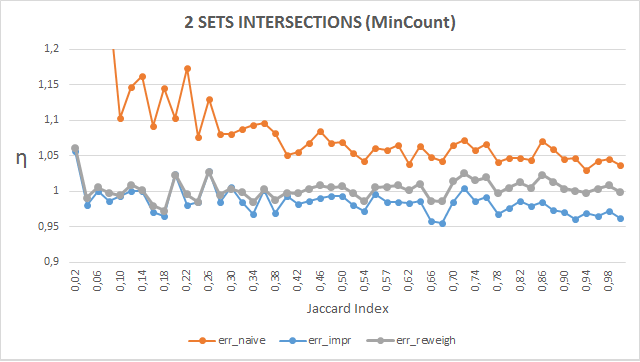
\includegraphics[width=0.6\textwidth]{KMV_2_sets_inter.png}
    \centering
    \caption{Porównanie metod dla przekrojów 2 zbiorów przy $n=10^5$}
    \label{fig:KMV_2sets_inter}
\end{figure}

\begin{figure}[h!]
    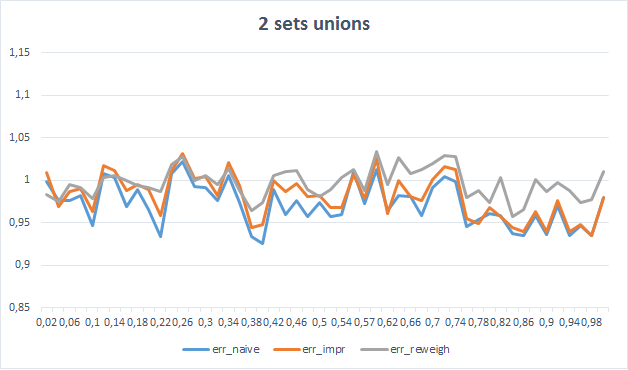
\includegraphics[width=0.6\textwidth]{KMV_2_sets_unions.png}
    \centering
    \caption{Porównanie metod dla sumy 2 zbiorów przy $n=10^5$}
    \label{fig:KMV_2sets_unions}
\end{figure}

Zauważmy, że dla operacji sumy - praktycznie na całym przedziale indeksów \textit{Jaccarda} zbiorów - najmniejszy błąd posiada metoda \textit{estymatora ważonego}. W przypadku przekroju - metody $2.$ oraz $3.$ wypadają o wiele lepiej niż metoda naiwna. Na wykresie możemy zauważyć, że metoda \textit{estymatora ważonego} posiada podobną tendencję jak metoda $2.$, ale dla większości indeksów \textit{Jaccarda} posiada mniejszy błąd.

Na kolejnych wykresach: \ref{fig:KMV_10sets_inter}, \ref{fig:KMV_10sets_unions}, \ref{fig:KMV_100sets_inter} oraz \ref{fig:KMV_100sets_unions}, zestawiliśmy wyniki dla sum i przekrojów większej liczby zbiorów. Wykonaliśmy eksperymenty dla 10 oraz 100 zbiorów o mocach $n = 10^5$, porównując metody $2.$ oraz $3.$ Metodę naiwną pominęliśmy ze względu na jej znaczące wady opisane w rozdziale \ref{naive_est}. 

Możemy zauważyć, że również jak na poprzednich wykresach dla dwóch zbiorów - metoda \textit{estymatora ważonego} posiada podobną tendencję jak metoda $2.$, ale również minimalizuje błąd - zwłaszcza dla dużych \textit{indeksów Jaccarda}.

\begin{figure}[h!]
    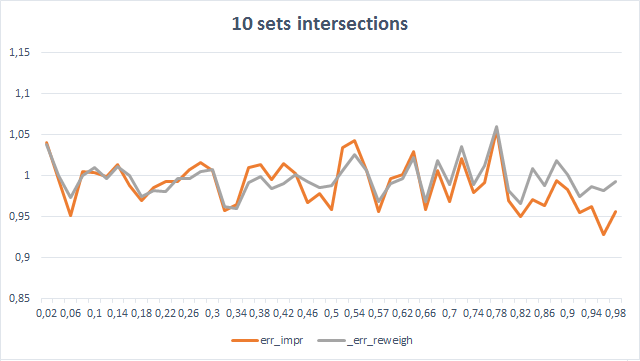
\includegraphics[width=0.6\textwidth]{KMV_10_sets_inter.png}
    \centering
    \caption{Porównanie metod dla przekroju 10 zbiorów}
    \label{fig:KMV_10sets_inter}
\end{figure}

\begin{figure}[h!]
    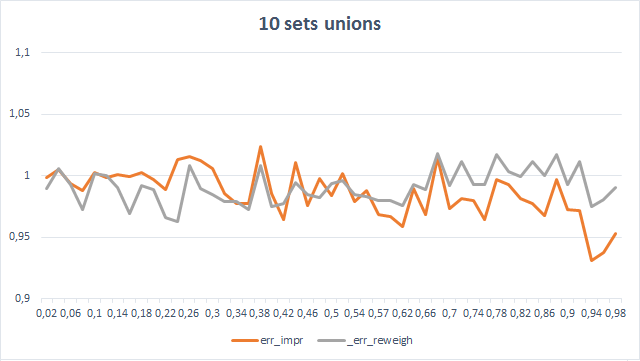
\includegraphics[width=0.6\textwidth]{KMV_10_sets_unions.png}
    \centering
    \caption{Porównanie metod dla sumy 10 zbiorów}
    \label{fig:KMV_10sets_unions}
\end{figure}

\begin{figure}[h!]
    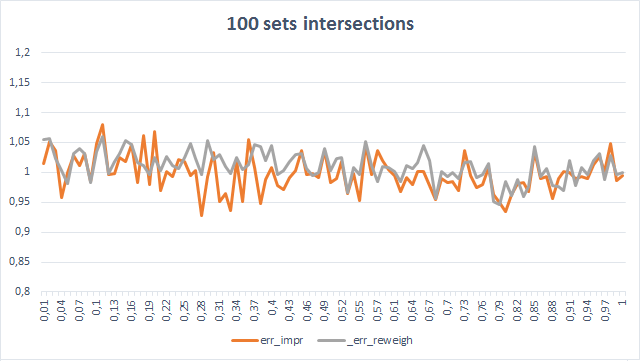
\includegraphics[width=0.6\textwidth]{KMV_100_sets_inter.png}
    \centering
    \caption{Porównanie metod dla przekroju 100 zbiorów}
    \label{fig:KMV_100sets_inter}
\end{figure}

\begin{figure}[h!]
    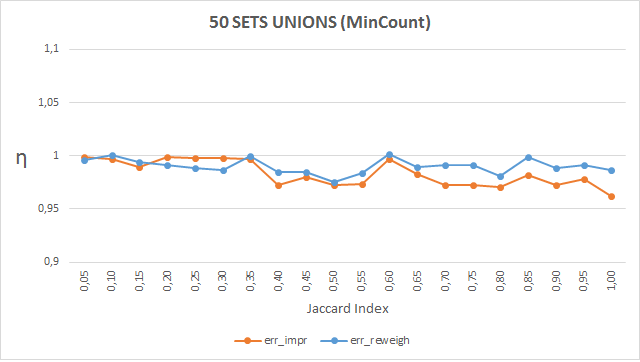
\includegraphics[width=0.6\textwidth]{KMV_100_sets_unions.png}
    \centering
    \caption{Porównanie metod dla sumy 100 zbiorów}
    \label{fig:KMV_100sets_unions}
\end{figure}

Ostatnimi eksperymentami przeprowadzonymi dla algorytmu \texttt{MinCount} było sprawdzenie metody \textit{estymatora ważonego} dla różnicy zbiorów, omówionej w rozdziale \ref{diff_weighted}. Na wykresie \ref{fig:KMV_2_sets_diff} przedstawiamy wyniki dla różnicy dwóch zbiorów, porównując podejście naiwne oraz podejście wykorzystujące \textit{estymator ważony}.

\begin{figure}[h!]
    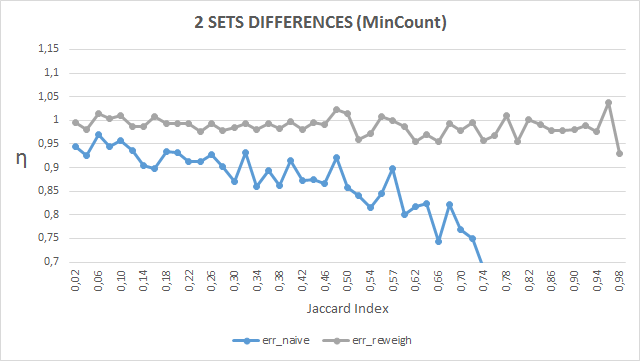
\includegraphics[width=0.6\textwidth]{KMV_2_sets_diff.png}
    \centering
    \caption{Porównanie metod dla różnicy 2 zbiorów}
    \label{fig:KMV_2_sets_diff}
\end{figure}

Zauważmy ze metoda \textit{estymatora ważonego} po raz kolejny wypada znacznie lepiej od metody naiwnej i utrzymuje mniej więcej stały błąd niezależnie od wartości \textit{indeksu Jaccarda} zbiorów. Nie możemy tego powiedzieć o metodzie naiwnej, której błąd znacznie rośnie wzrast z wzrostem podobieństwa zbiorów.

\newpage
\section{Wyniki dla algorytmu HyperLogLog}
%\AW{przez noc wygeneruje jeszcze dokladniejsze wykresy dla HLL}
W tym podrozdziale przedstawimy wyniki dla algorytmu \texttt{HyperLogLog}. Zestawiliśmy ze sobą dwie metody:
\begin{enumerate}
	\item metoda naiwna z użyciem indeksu \textit{Jaccarda} (wzór (\ref{jacc_1}))
	\item metoda \textit{estymatora ważonego}
\end{enumerate}
Obydwie metody korzystają z pomocniczej struktury dla każdego ze szkiców, przechowującej $k$ najmniejszych wartości (czyli zasadniczo z podstawowej wersji szkicu \texttt{MinCount}), pozwalającej na estymację indeksu \textit{Jaccarda} \cite{adroll}, potrzebnego zarówno do estymacji metodą naiwną jak i metodą \textit{estymatora ważonego}. W przeprowadzanych eksperymentach ustaliliśmy parametry $k = 80$ oraz $p = 8$.
Na wykresach przedstawiamy wartości $\eta = \frac{\hat{n}}{n}$ dla poszczególnych metod, oznaczone na legendzie przez odpowiednio:
\begin{enumerate}
	\item \textbf{err\_naive}
	\item \textbf{err\_reweigh}
\end{enumerate}

Na wykresach \ref{fig:HLL_2_sets_unions}, \ref{fig:HLL_2_sets_unions}, \ref{fig:HLL_10_sets_unions} oraz \ref{fig:HLL_10_sets_inter} przedstawiamy porównanie powyższych metod w kontekście operacji sumy oraz przekroju. Eksperymenty przeprowadziliśmy dla 2 oraz 10 zbiorów o mocach $n=10^5$.

\begin{figure}[h!]
	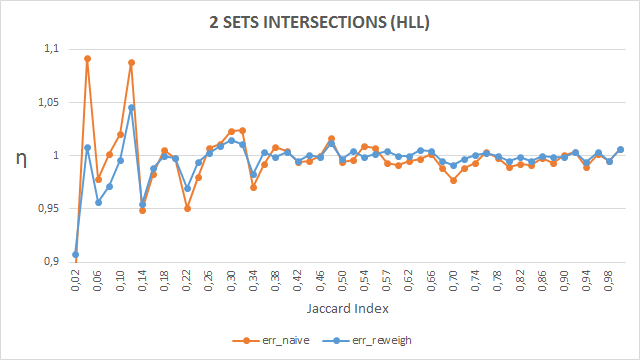
\includegraphics[width=0.6\textwidth]{HLL_2_sets_inter.png}
	\centering
	\caption{Porównanie metod dla przekroju 2 zbiorów przy $n=10^5$}
	\label{fig:HLL_2_sets_inter}
\end{figure}

\begin{figure}[h!]
	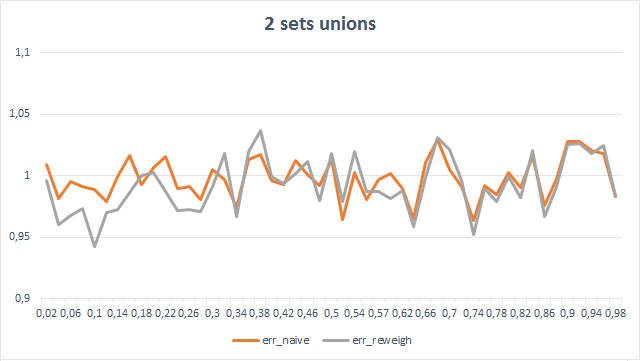
\includegraphics[width=0.6\textwidth]{HLL_2_sets_unions.png}
	\centering
	\caption{Porównanie metod dla sumy 2 zbiorów przy $n=10^5$}
	\label{fig:HLL_2_sets_unions}
\end{figure}

\begin{figure}[h!]
    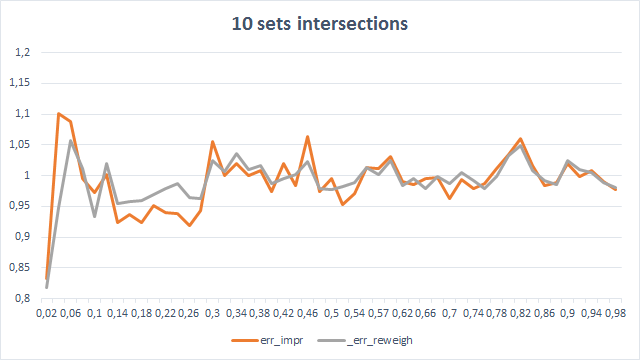
\includegraphics[width=0.6\textwidth]{HLL_10_sets_inter.png}
    \centering
    \caption{Porównanie metod dla przekroju 10 zbiorów przy $n=10^5$}
    \label{fig:HLL_10_sets_inter}
\end{figure}
\AW{tutaj jest blad w legendzie na wykresie - powinno byc err\_naive zamiast err\_impr!}

\begin{figure}[h!]
    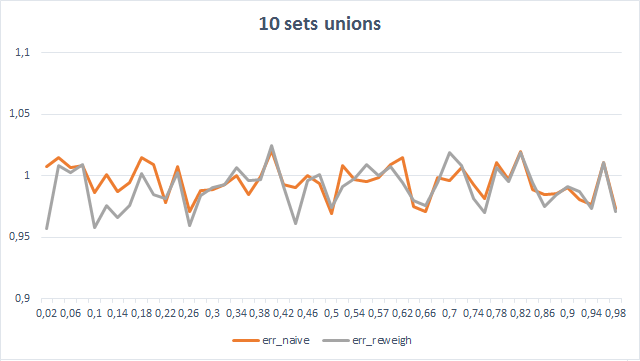
\includegraphics[width=0.6\textwidth]{HLL_10_sets_unions.png}
    \centering
    \caption{Porównanie metod dla sumy 10 zbiorów przy $n=10^5$}
    \label{fig:HLL_10_sets_unions}
\end{figure}

Wnioski wynikające z tych eksperymentów sugerują, że metoda \textit{estymatora ważonego} w kontekście algorytmu \texttt{HyperLogLog} dla operacji sumy niestety nie dorównuje pod względem dokładności podejściu naiwnemu. W przypadku sumy jest to dosyć oczywiste, ponieważ jak wspominaliśmy w rozdziale 2 - \texttt{HyperLogLog} posiada naturalną operację sumy. W przypadku operacji przekroju metoda naiwna wykorzystująca indeks \textit{Jaccarda} i wzór (\ref{jacc_1}) posiada większy błąd niż estymacja z użyciem \textit{estymatora ważonego}, zwłaszcza dla zbiorów o niskim podobieństwie. Zauważmy że obie metody wykorzystują tyle samo pamięci, bowiem obie wymagają dodatkowej struktury pozwalającej na estymację indeksu \textit{Jaccarda} przy wykorzystaniu algorytmu \texttt{MinHash}.

\section{Porównanie algorytmów Streaming MinCount i HyperLogLog}

W tym podrozdziale przedstawiamy wyniki porównania algorytmów \texttt{Streaming MinCount} oraz \texttt{HyperLogLog}. Aby porównać oba algorytmy, dopasowaliśmy ich parametry tak, aby oba algorytmy wykorzystywały tą sama ilość pamięci. Na wykresach \ref{fig:HLL_KMV_2_sets_unions} oraz \ref{fig:HLL_KMV_10_sets_unions} przedstawiamy porównanie wartości $\eta = \frac{\hat{n}}{n}$ najlepszych metod dla poszczególnych algorytmów w kontekście operacji sumowania, przy liczności testowych zbiorów $n=10^5$:
\begin{enumerate}
	\item metoda \textit{estymatora ważonego} dla algorytmu \texttt{Streaming MinCount} - \textbf{err\_MC}
	\item naturalna metoda sumowania dla algorytmu \texttt{HyperLogLog} (zobacz \ref{HLL_sum}) - \textbf{err\_HLL}
\end{enumerate}

\begin{figure}[h!]
	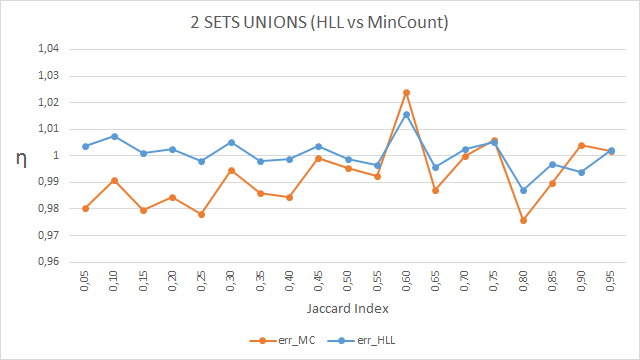
\includegraphics[width=0.6\textwidth]{HLL_KMV_2_sets_unions.png}
	\centering
	\caption{Porównanie algorytmów dla sumy 2 zbiorów przy $n=10^5$}
	\label{fig:HLL_KMV_2_sets_unions}
\end{figure}

\begin{figure}[h!]
	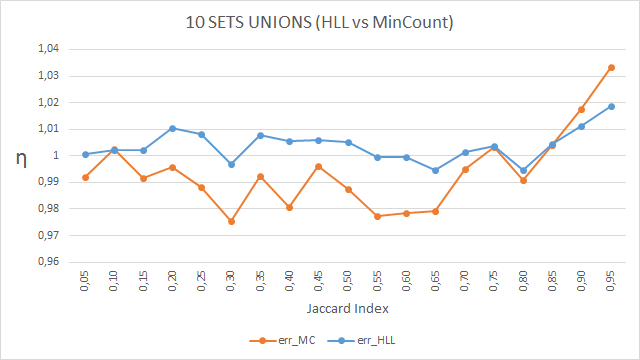
\includegraphics[width=0.6\textwidth]{HLL_KMV_10_sets_unions.png}
	\centering
	\caption{Porównanie algorytmów dla sumy 10 zbiorów przy $n=10^5$}
	\label{fig:HLL_KMV_10_sets_unions}
\end{figure}
W przypadku operacji sumowania zbiorów, algorytm \texttt{HyperLogLog} wypada zdecydowanie lepiej, zwłaszcza dla większej liczby zbiorów. Ta obserwacja utwierdza nas w przekonaniu że naturalna operacjia sumy, którą posiada szkic algorytmu \texttt{HyperLogLog} jest najefektywniejsza i jak wynika z naszych eksperymentów - sprawdza sie lepiej niż algorytm \texttt{Streaming MinCount}, przy takim samym wykorzystaniu pamięci.

Na wykresach \ref{fig:HLL_KMV_2_sets_inter} oraz \ref{fig:HLL_KMV_10_sets_inter} przedstawiamy porównanie wartości $\eta = \frac{\hat{n}}{n}$ najlepszych metod dla poszczególnych algorytmów w kontekście operacji przekroju, przy liczności testowych zbiorów $n=10^5$:
\begin{enumerate}
	\item metoda \textit{estymatora ważonego} dla algorytmu \texttt{Streaming MinCount} - \textbf{err\_MC}
	\item metoda \textit{estymatora ważonego} dla algorytmu \texttt{HyperLogLog} - \textbf{err\_HLL}
\end{enumerate}

\begin{figure}[h!]
	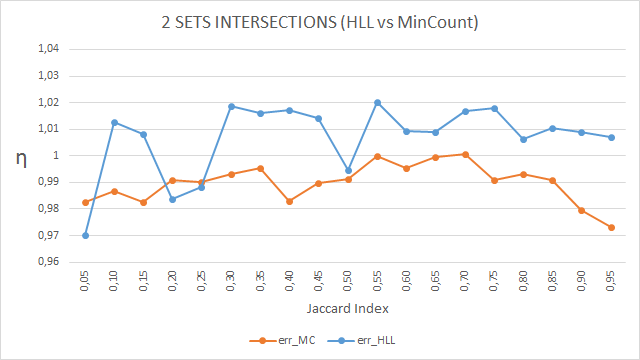
\includegraphics[width=0.6\textwidth]{HLL_KMV_2_sets_inter.png}
	\centering
	\caption{Porównanie algorytmów dla przekroju 2 zbiorów przy $n=10^5$}
	\label{fig:HLL_KMV_2_sets_inter}
\end{figure}

\begin{figure}[h!]
	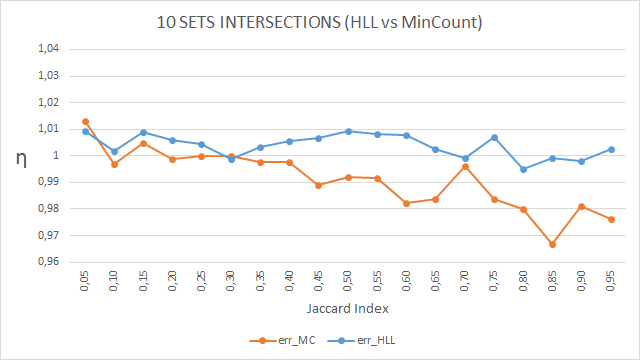
\includegraphics[width=0.6\textwidth]{HLL_KMV_10_sets_inter.png}
	\centering
	\caption{Porównanie algorytmów dla przekroju 10 zbiorów przy $n=10^5$}
	\label{fig:HLL_KMV_10_sets_inter}
\end{figure}

W przypadku przekrojów sytuacja nie jest tak oczywista jak dla sumy. Dla dwóch zbiorów, wyniki sugerują, że algorytmy sprawują się porównywalnie - z niewielką przewaga algorytmu \texttt{Streaming MinCount} na przedziale indeksów \textit{Jaccarda} od ok $0.20$ do $0.85$. Jednak symulacje dla 10 zbiorów już wykazują, że algorytmy zachowuja się podobnie gdy podobieństwo zbiorów jest mniejsze niż $0.50$. Jednak dla większych indeksów \textit{Jaccarda} przewagę uzyskuje algorytm \texttt{HyperLogLog}.


	\cleardoublepage
	
	\chapter{Podsumowanie}
\thispagestyle{chapterBeginStyle}

W pracy podjęliśmy problem
%JL naszej 
%JL zajęliśmy się problemem zliczania unikalnych elementów w strumieniach danych 
%JL a konkretnie
efektywnego wykonywania operacji teoriomnogościowych na szkicach danych algorytmów \texttt{MinCount} oraz \texttt{HyperLogLog}.
Omówiliśmy i przedstawiliśmy naiwne metody estymacji dla operacji teoriomnogościowych jak i nowe metody zaproponowane w pracy \cite{ting} dla algorytmu \texttt{MinCount}, skupiając się na metodzie \textit{estymatora ważonego}, która zdaniem autorów pod względem efektywności jest zbliżona do estymatora wyprowadzonego metodą \textit{największej wiarygodności}. Następnie rozwinęliśmy 
%JL definicję 
metodę
\textit{estymatora ważonego} dla operacji różnicy oraz przedstawiliśmy pomysł generalizacji tej metody dla algorytmu \texttt{HyperLogLog}, wykorzystując do tego algorytm pomocniczy \texttt{MinHash}.

Nasze teoretyczne rozważania podsumowaliśmy przedstawiając wyniki eksperymentów mających na celu weryfikację powyższych metod w praktyce. Nasze eksperymenty potwierdziły, że metoda \textit{estymatora ważonego} w większości przypadków posiada najmniejszy błąd. Eksperymenty pokazały również, że nasza idea zastosowania metody \textit{estymatora ważonego} w algorytmie \texttt{HyperLogLog} poprawia wyniki estymacji przekroju dla tego algorytmu.
%JL czego nie można powiedzieć o operacji sumy, która będąc naturalnie wbudowana w szkic algorytmu \texttt{HyperLogLog}, skutkuje największa dokładnością.

Na koniec porównaliśmy ze sobą oba algorytmy \texttt{MinCount} oraz \texttt{HyperLogLog} w kontekście operacji teoriomnogościowych, dla każdego z nich wybierając najefektywniejszą metodę estymacji dla danej operacji. Wyniki wykazały, że dla większej liczby zbiorów, zarówno dla operacji sumy jak i przekroju - algorytm \texttt{HyperLogLog} posiada najlepszą dokładność estymacji.
%\JL{Powyższe zdanie - myslałem, że dla sumy nie używamy estymatora ważonego??}




	\cleardoublepage
	
	
	%%%%%%%%%%%%%%%%%%%%%%%%%%%%%%%%%%%%%%%%%%%%%%%%%%%%%%%%%%%%%%%%%%%%%%%%%%%%%%
	%%%%%%%%%%%%%%%%%%%%%%%%%%%%%%% BIBLIOGRAFIA %%%%%%%%%%%%%%%%%%%%%%%%%%%%%%%%%
	%%%%%%%%%%%%%%%%%%%%%%%%%%%%%%%%%%%%%%%%%%%%%%%%%%%%%%%%%%%%%%%%%%%%%%%%%%%%%%

	\pagestyle{bibliographyStyle}
	\bibliographystyle{plabbrv}
	\bibliography{literatura}
	\thispagestyle{chapterBeginStyle}
        \addcontentsline{toc}{chapter}{Bibliografia}

	\cleardoublepage
	
	%%%%%%%%%%%%%%%%%%%%%%%%%%%%%%%%%%%%%%%%%%%%%%%%%%%%%%%%%%%%%%%%%%%%%%%%%%%%%%
	%%%%%%%%%%%%%%%%%%%%%%%%%%%%%%%%% DODATKI %%%%%%%%%%%%%%%%%%%%%%%%%%%%%%%%%%%%
	%%%%%%%%%%%%%%%%%%%%%%%%%%%%%%%%%%%%%%%%%%%%%%%%%%%%%%%%%%%%%%%%%%%%%%%%%%%%%%
	
	\appendix
	\pagestyle{appendixStyle}
	
	\chapter{Zawartość płyty CD}
\thispagestyle{chapterBeginStyle}
\label{plytaCD}

W tym rozdziale należy krótko omówić zawartość dołączonej płyty CD.


	\cleardoublepage

\end{document}

